\documentclass[conference]{IEEEtran}
\IEEEoverridecommandlockouts

\usepackage{cite}
\usepackage{amsmath,amssymb,amsfonts}
\usepackage{algorithmic}
\usepackage{graphicx}
\usepackage{textcomp}
\usepackage{xcolor}
\def\BibTeX{{\rm B\kern-.05em{\sc i\kern-.025em b}\kern-.08em
    T\kern-.1667em\lower.7ex\hbox{E}\kern-.125emX}}
\begin{document}

\title{Assignment Report}

\author{\IEEEauthorblockN{ Vamshi Krishna Edamadaka}
\IEEEauthorblockA{\textit{Computer Science} \\
\textit{University of North Carolina Greensboro}\\
Greensboro, USA \\
v\textunderscore edamadaka@uncg.edu}
}

\maketitle
\section{Assignment 01: Raw Data to Feature Space}
\section{TASK 1 }
\subsection{Building your own programming environment!}
Installing the IDE on our different PCs is the first step in creating a programming environment. The instructions for installing the Anaconda environment on a PC are as follows.
\begin{enumerate}
    \item 
   Go to https://docs.anaconda.com/anaconda/[1] for further information. Then, on the left, click the 'Installation' tab.

    \item Choose the operating system on which Anaconda will be installed. I click the 'Installing on Windows' link to install Anaconda on my local machine.

\item Download the Anaconda Installer onto your local environment.
\begin{figure}[!htbp]
    \centering
    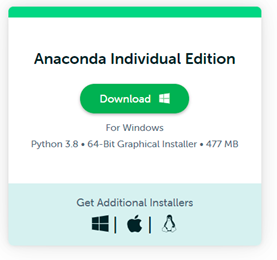
\includegraphics[height=4cm]{Task1 Step3.png}
   
    \label{fig:my_label}
\end{figure}
\begin{figure}[!htbp]
    \centering
    
\end{figure}

 \item To run the application, double-click the installer and then select 'Next.'
\begin{figure}[!htbp]
    \centering
    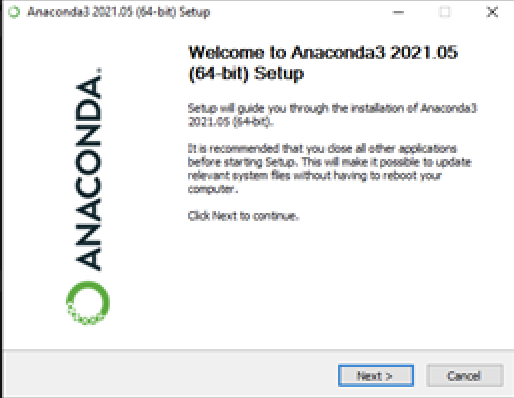
\includegraphics[height=4cm]{task4.png}
   
    \label{fig:my_label}
\end{figure}
\begin{figure}[!htbp]
    \centering
    
\end{figure}



\item Read the License Agreement and the click on ‘I Agree’.
\begin{figure}[!htbp]
    \centering
    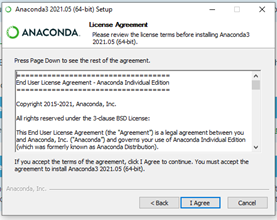
\includegraphics[height=4cm]{Task1 Step5.png}
   
    \label{fig:my_label}
\end{figure}
\begin{figure}[!htbp]
    \centering
    
\end{figure}

\item Then, for the installation type, select 'Just Me,' as we are simply configuring the environment for the local user. Then press the 'Next' button.
\begin{figure}[!htbp]
    \centering
    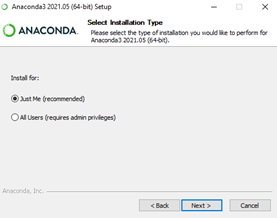
\includegraphics[height=4cm]{Task1 Step6.png}
   
    \label{fig:my_label}
\end{figure}
\begin{figure}[!htbp]
    \centering
    
\end{figure}

\item
Select a destination folder in which to install Anaconda.
\begin{figure}[!htbp]
    \centering
    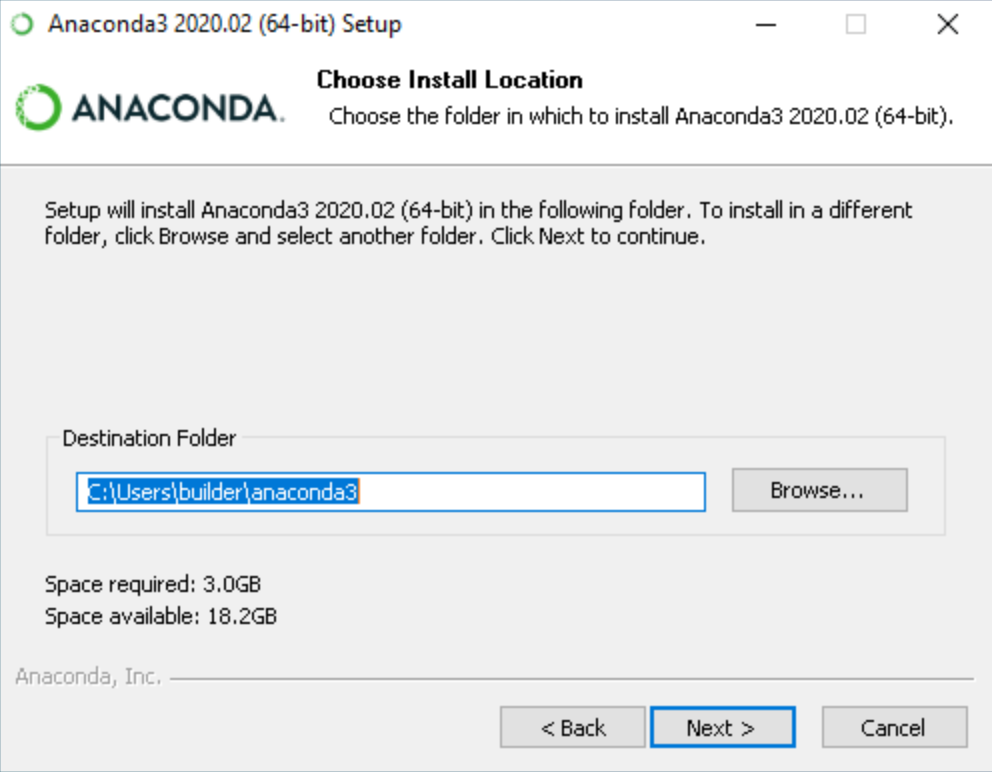
\includegraphics[height=4cm]{task7.png}
   
    \label{fig:my_label}
\end{figure}
\begin{figure}[!htbp]
    \centering
    
\end{figure}
\item
To avoid any conflicts with other applications installed on your computer, select 'Register Anaconda3 as my default Python 3.8' from the advanced installation menu. Then press the 'Install' button.
\begin{figure}[!htbp]
    \centering
    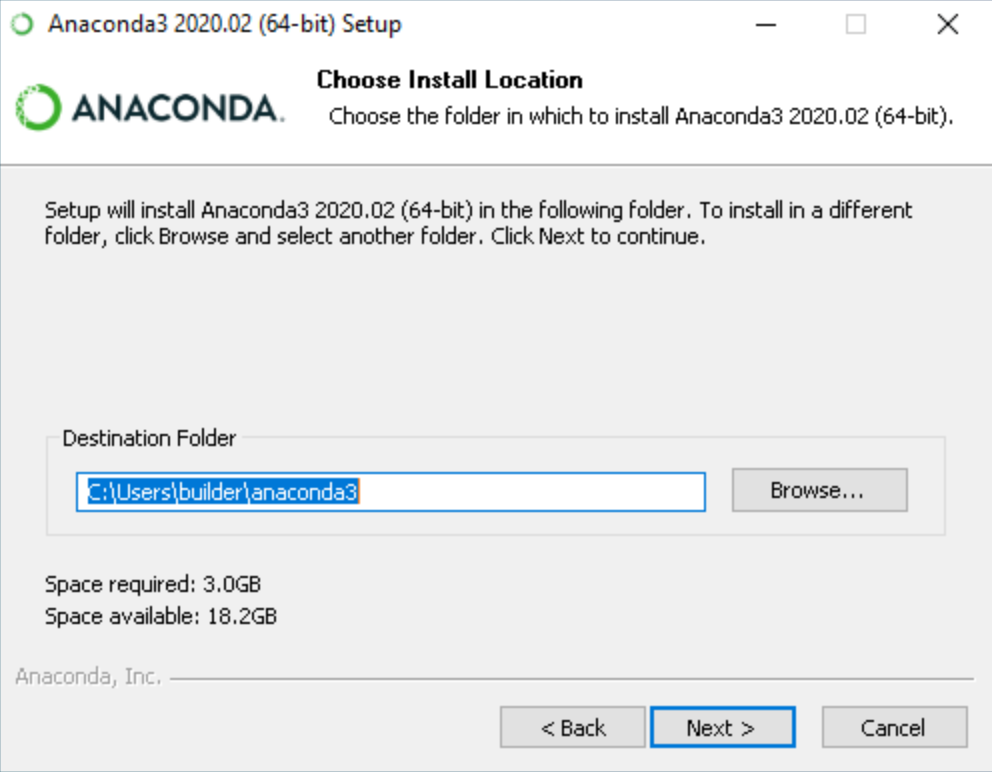
\includegraphics[height=4cm]{task7.png}
   
    \label{fig:my_label}
\end{figure}
\begin{figure}[!htbp]
    \centering
    
\end{figure}

\item 
After installation is complete, click on ‘Next’.
\begin{figure}[!htbp]
    \centering
    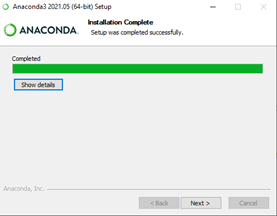
\includegraphics[height=4cm]{Task1 Step9.png}
   
    \label{fig:my_label}
\end{figure}
\begin{figure}[!htbp]
    \centering
    
\end{figure}

\item
The Thank You for installation dialog box appears after successful completion. Here click ‘Finish’
\begin{figure}[!htbp]
    \centering
    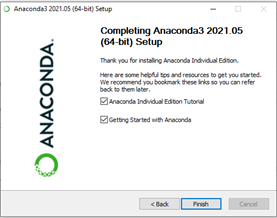
\includegraphics[height=4cm]{Task1 Step10.png}
   
    \label{fig:my_label}
\end{figure}
\begin{figure}[!htbp]
    \centering
    
\end{figure}
 \\Anaconda is now successfully built onto your local environment.

\end{enumerate}

\subsection {Install the Spyder IDE}

Spyder[2], or the Scientific Python Development Environment, is a powerful open-source integrated development environment (IDE) created in Python for Python. Anaconda comes with a free integrated development environment (IDE).

Opening Anaconda and selecting the Spyder IDE by clicking on 'launch' is one approach to start Spyder.

Spyder can be be launched by typing'spyder' into the Anaconda Prompt.
\subsection {Installing OpenCV}

The OpenCV-Python library is a set of Python bindings for solving computer vision issues. Numpy, a highly efficient library for numerical operations with a MATLAB-style syntax, is used by OpenCV-Python. Numpy arrays are translated to and from all OpenCV array forms.

To install the OpenCV package, start a command line and run the following command after navigating to the Anaconda installation folder: \\

pip install opencv-python \\


\section{TASK 2}
\subsection{Download or generate a fruit and vegetables image datasets!}
\begin{enumerate}
    \item The datasets are obtained from the following website[3]: \\ "https://www.vicos.si/Downloads/FIDS30"
   
\item The apple, mango, and strawberry were chosen as the three fruits for this task.

\begin{figure}[!htbp]
    \centering
    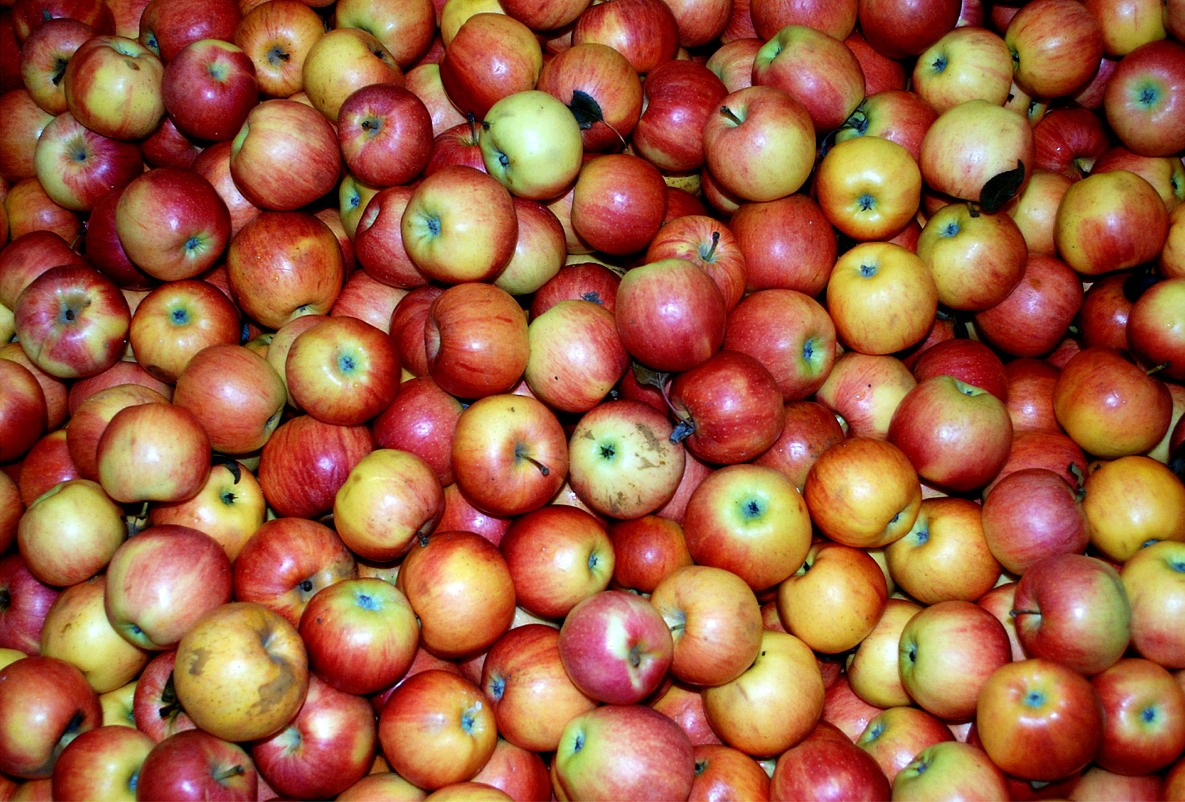
\includegraphics[height=2cm]{apple.jpg}
    \caption{apple}
    \label{fig:my_label}
\end{figure}
\begin{figure}[!htbp]
    \centering
    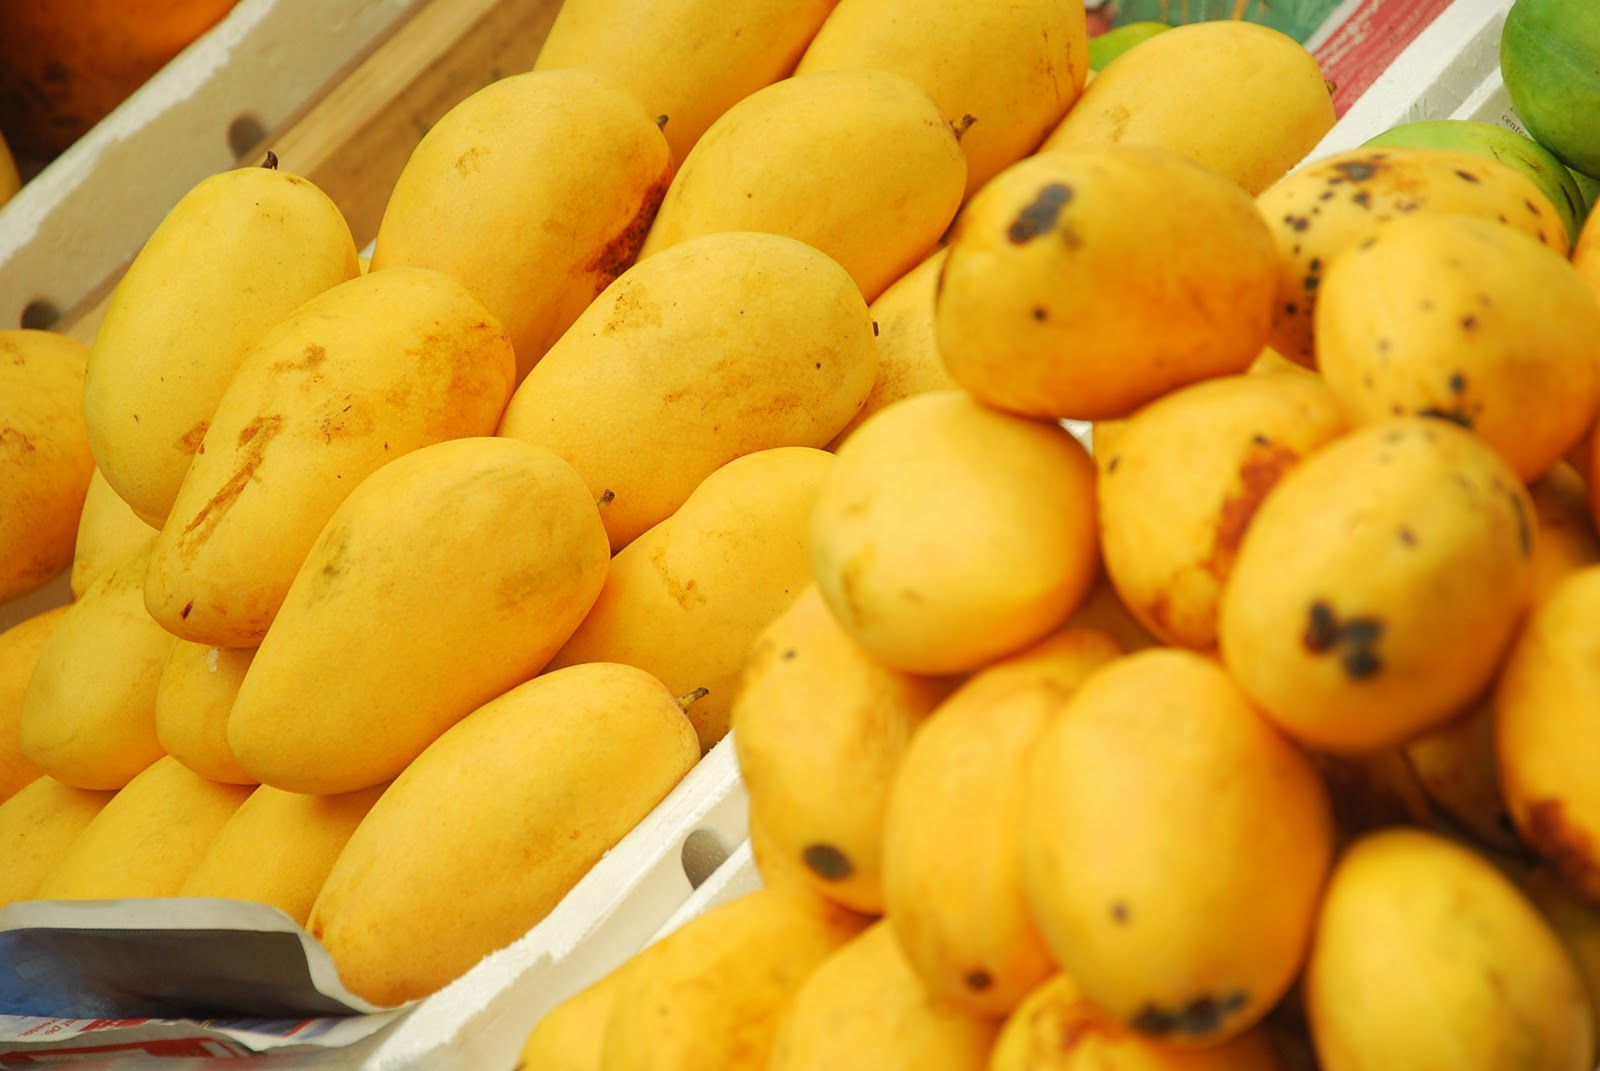
\includegraphics[height=2cm]{mango.jpg}
    \caption{mango}
    \label{fig:my_label}
\end{figure}
\begin{figure}[!htbp]
    \centering
    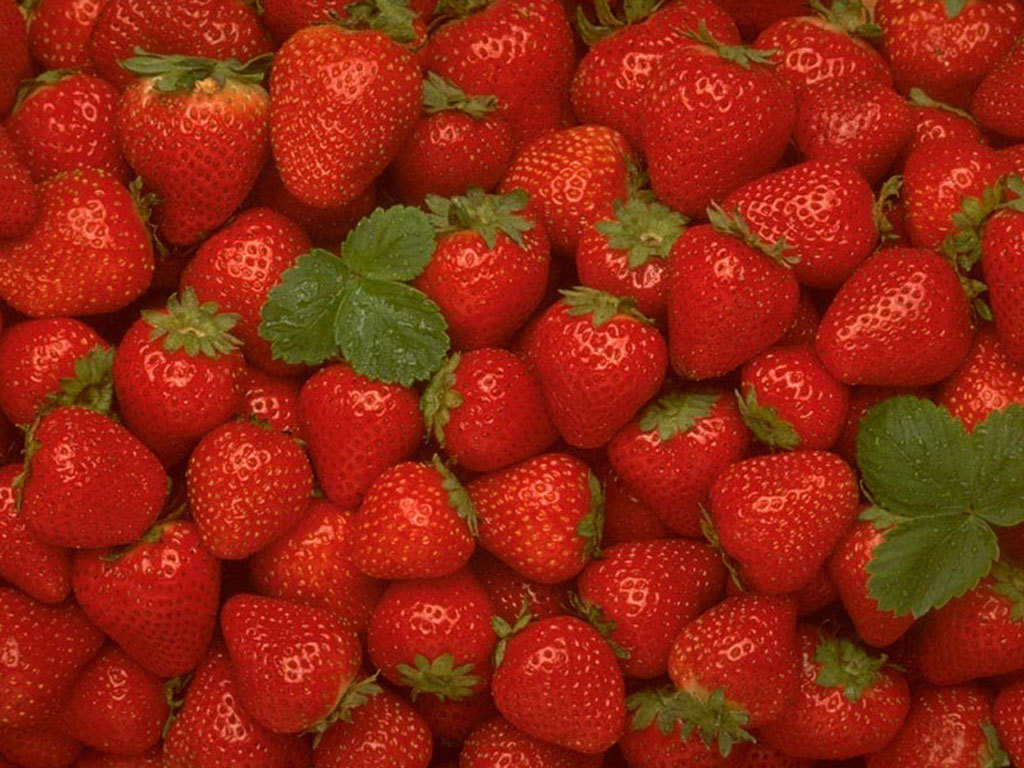
\includegraphics[height=2cm]{strawberry.jpg}
    \caption{strawberry}
    \label{fig:my_label}
\end{figure}
\end{enumerate}


\section{Task 3}
\subsection{Write a simple code to read your selected images and display them on the environment!}
To perform this particular task we import the following libraries:

\begin{figure}[!htbp]
    \centering
    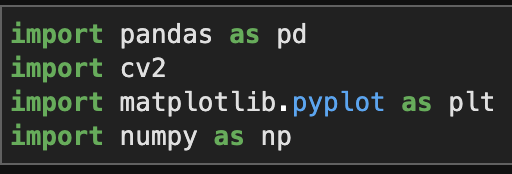
\includegraphics[height=2cm]{import.png}
      \caption{Import statements}
  \label{fig:Apple-RBG }
  \end{figure}
  
Apple, mango, and strawberry are the three fruits chosen for this project:\\
\begin{figure}[!htbp]
    \centering
    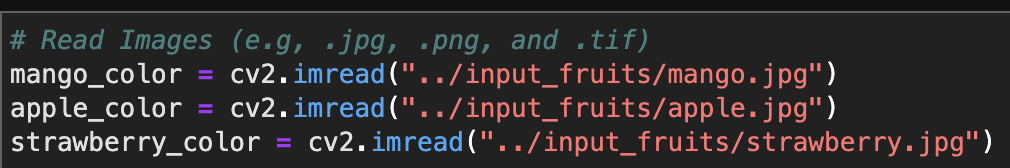
\includegraphics[width=10cm]{image upload.png}
     \caption{importing the images}
  \label{fig:Strawberry-RBG }
    
\end{figure}
We are now going to plot their R, G, and B channel images.
\begin{figure}[!htbp]
    \centering
    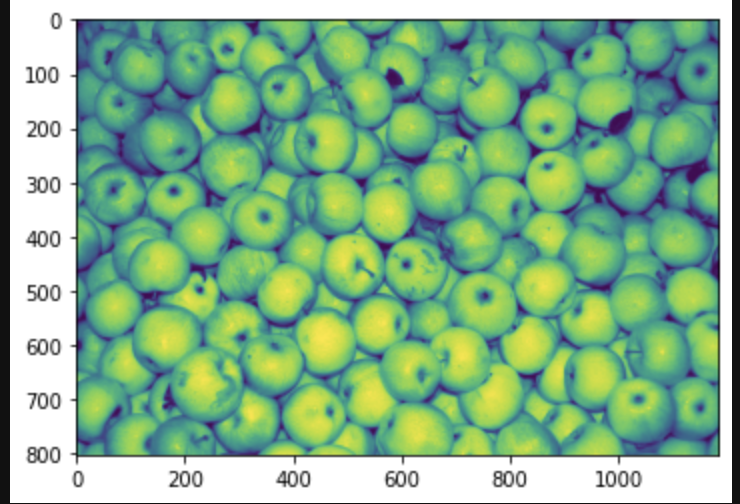
\includegraphics[height=3cm]{apple_rgb.png}
      \caption{Apple-RBG}
  \label{fig:Apple-RBG }
   
\end{figure}

\begin{figure}[!htbp]
    \centering
    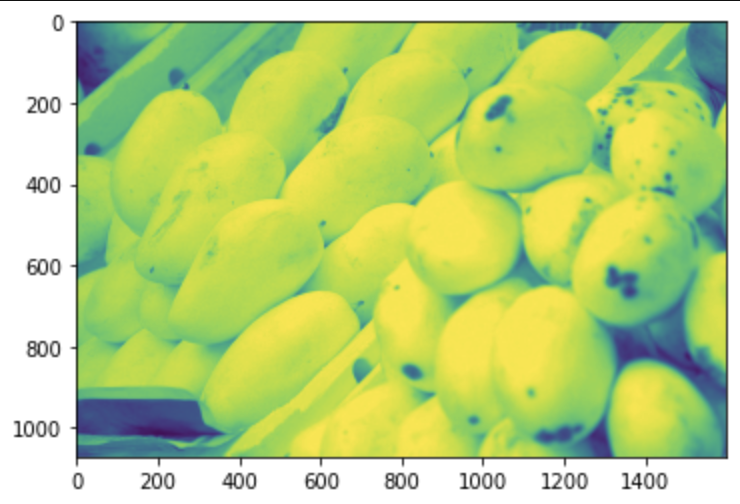
\includegraphics[height=3cm]{mango_rgb.png}
      \caption{mango-RBG}
  \label{fig:mango-RBG }
    
\end{figure}


\begin{figure}[!htbp]
    \centering
    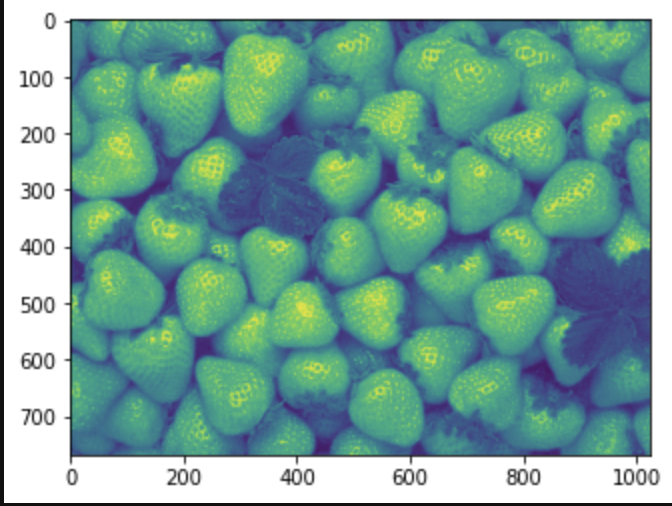
\includegraphics[height=3cm]{strawberry_rgb.png}
     \caption{Strawberry-RBG}
  \label{fig:Strawberry-RBG }
    
\end{figure}
\subsection{Convert these color images to grayscale and display them while printing their dimensions}

The color photos that have been made can be turned to grayscale and shown while being printed in their original dimensions. When photographs are converted to grey scale, their dimensions are printed.



\begin{figure}[!htbp]
    \centering
    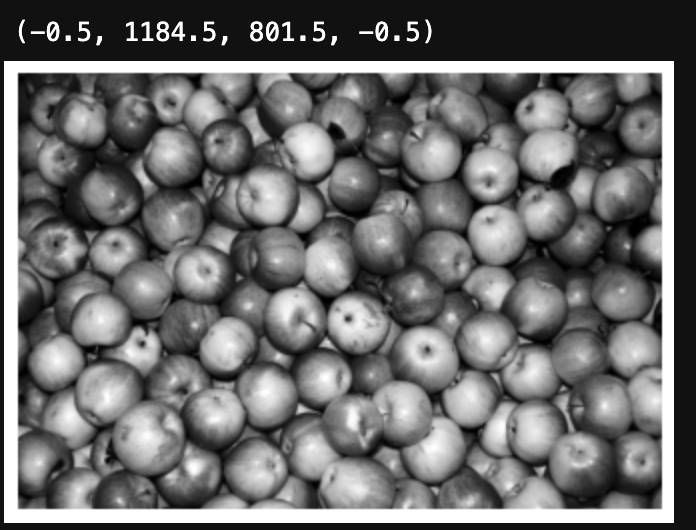
\includegraphics[height=3cm]{apple_bw.png}
     \caption{apple greyscale with dimensions (-0.5, 1184.5, 801.5, -0.5)}
  \label{fig:AppleGrey}
   
\end{figure}

\begin{figure}[!htbp]
    \centering
    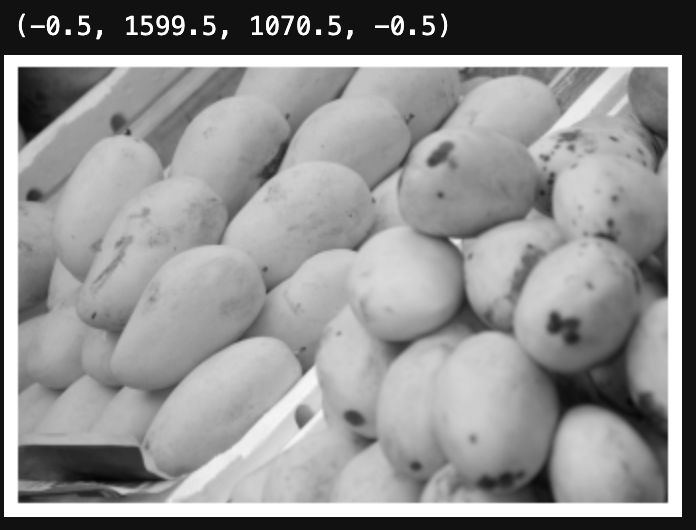
\includegraphics[height=3cm]{mango_bw.png}
     \caption{mango greyscale with Dimensions (-0.5, 1599.5, 1070.5, -0.5)}
  \label{fig:AppleGrey Dimension }
    
\end{figure}

\begin{figure}[!htbp]
    \centering
    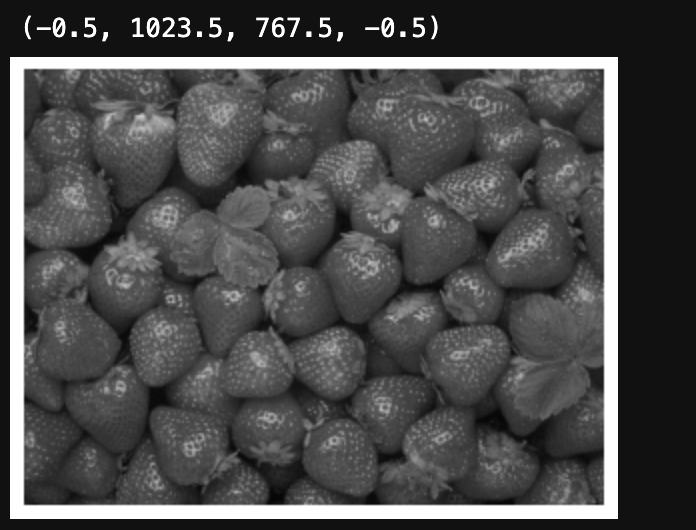
\includegraphics[height=3cm]{strawberry_bw.png}
   \caption{strawberry with dimensions (-0.5, 1023.5, 767.5, -0.5) }
  \label{fig:mangoGrey  }
    \label{fig:my_label}
\end{figure}


\section{Task 4}
\subsubsection{Resize the images to reduce their dimensions!}\\
We'll downsize the photographs in this work to make them smaller. The picture resizing is done here so that we can extract features from the image faster and utilize them to train our models later. \\
The resized images will produce the following output:

\begin{figure}[!htbp]
    \centering
    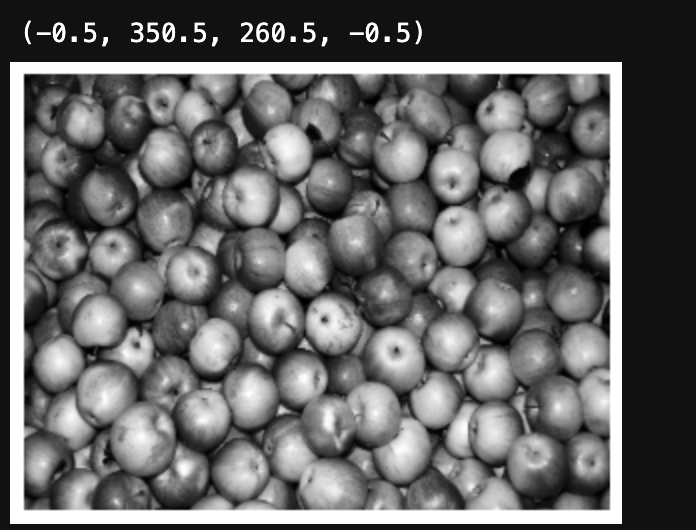
\includegraphics[height=3cm]{apple_resized.png} 
     \caption{Apple-Resized to (-0.5, 350.5, 260.5, -0.5)}
  \label{fig:AppleGray-Resized}
   
\end{figure}

\begin{figure}[!htbp]
    \centering
    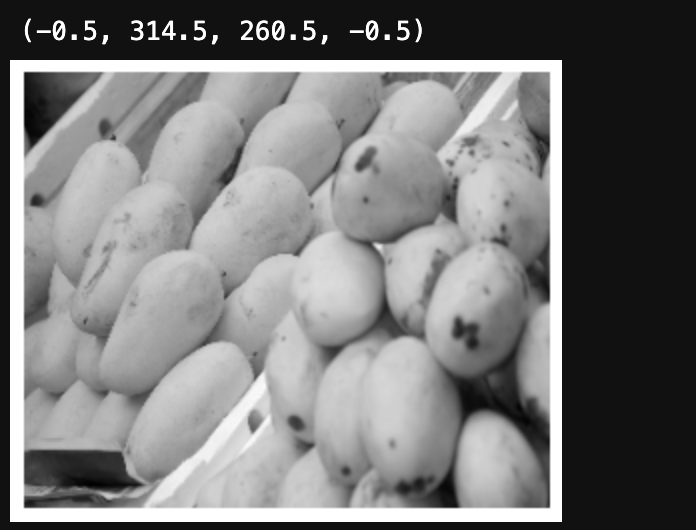
\includegraphics[height=3cm]{mango_resized.png}
   \caption{Mango-Resized to (-0.5, 314.5, 260.5, -0.5)}
  \label{fig:AppleGray-Resized Dimension}
   
\end{figure}

\begin{figure}[!htbp]
    \centering
    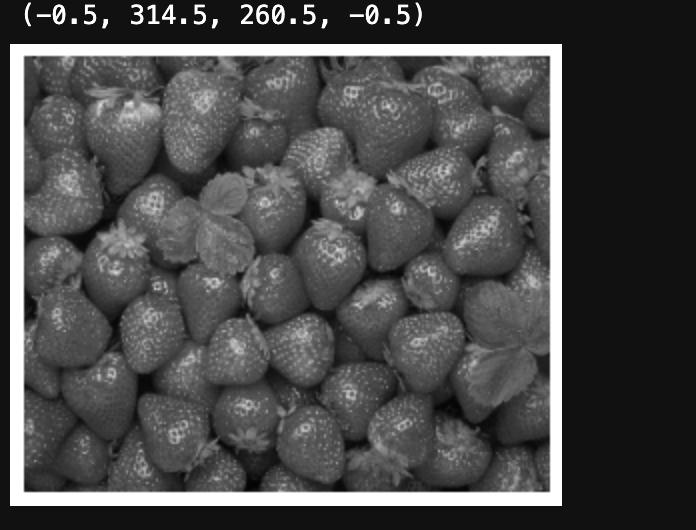
\includegraphics[height=3cm]{strawberry_resized.png} 
    \caption{Strawberry-Resized to (-0.5, 314.5, 260.5, -0.5) }
  \label{fig:mangoGray-Resized }
    
\end{figure}

\section{Task 5}
\subsection{Generate block-feature vectors!}
Now we'll build code to partition an image into 9x9 pixel sliding blocks, convert them to 81-bit vectors, and label each feature vector with 0, 1, and 2 for the first, second, and third images, respectively. Then, for each image, we create a spreadsheet by saving a feature vector per row in the spreadsheet. \\
\begin{figure}[!htbp]
    \centering
    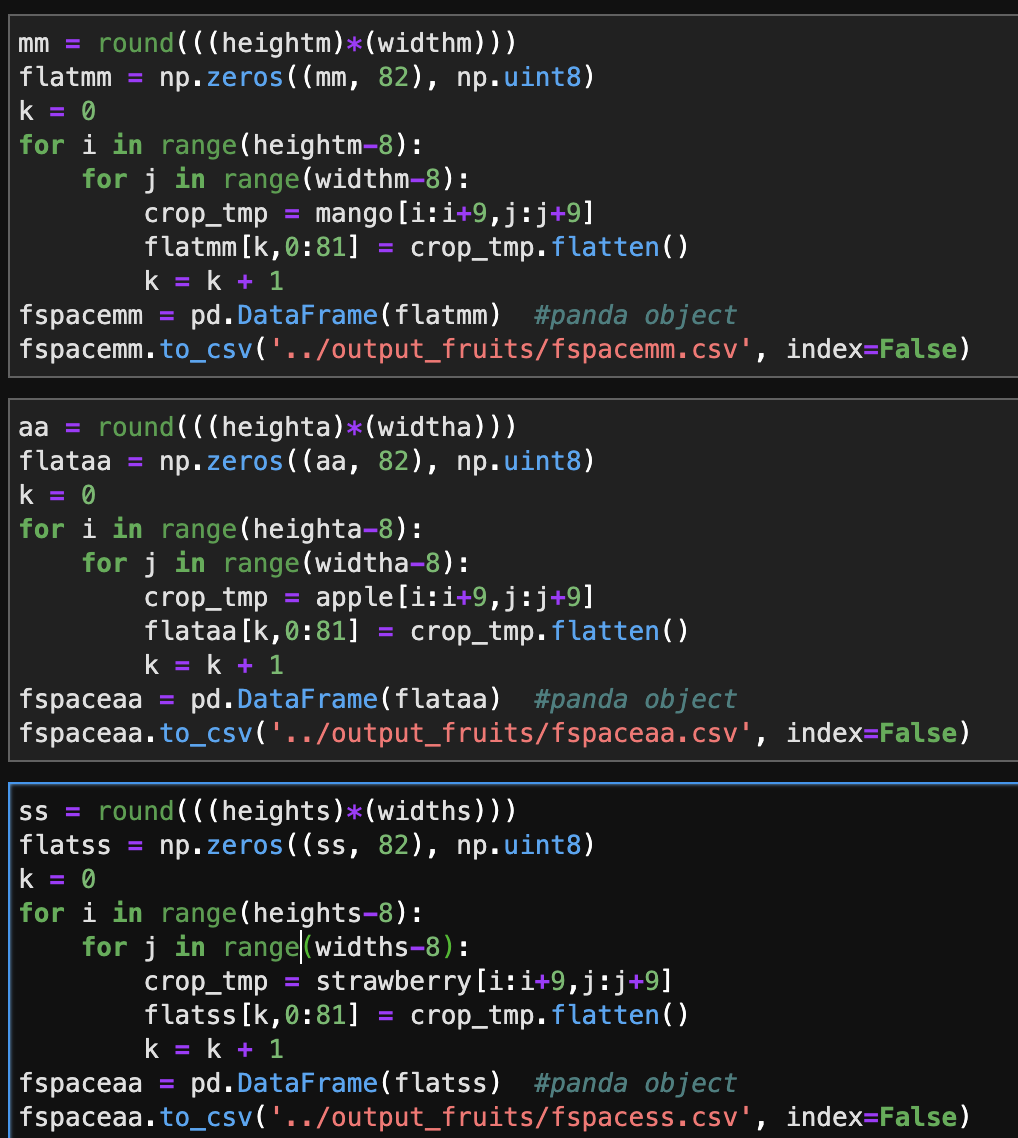
\includegraphics[height=9cm]{task5.png} 
    \caption{Task 5 }
  \label{fig:mangoGray-Resized }
    
\end{figure}


\section{Task 6}
\subsection{Generate sliding block-feature vectors!}
Now we'll build code to partition an image into 9x9 pixel sliding blocks, convert them to 81-bit vectors, and label each feature vector with 0, 1, and 2 for the first, second, and third images, respectively. Then, for each image, we create a spreadsheet by saving a feature vector per row in the spreadsheet. \\\\
\begin{figure}[!htbp]
    \centering
    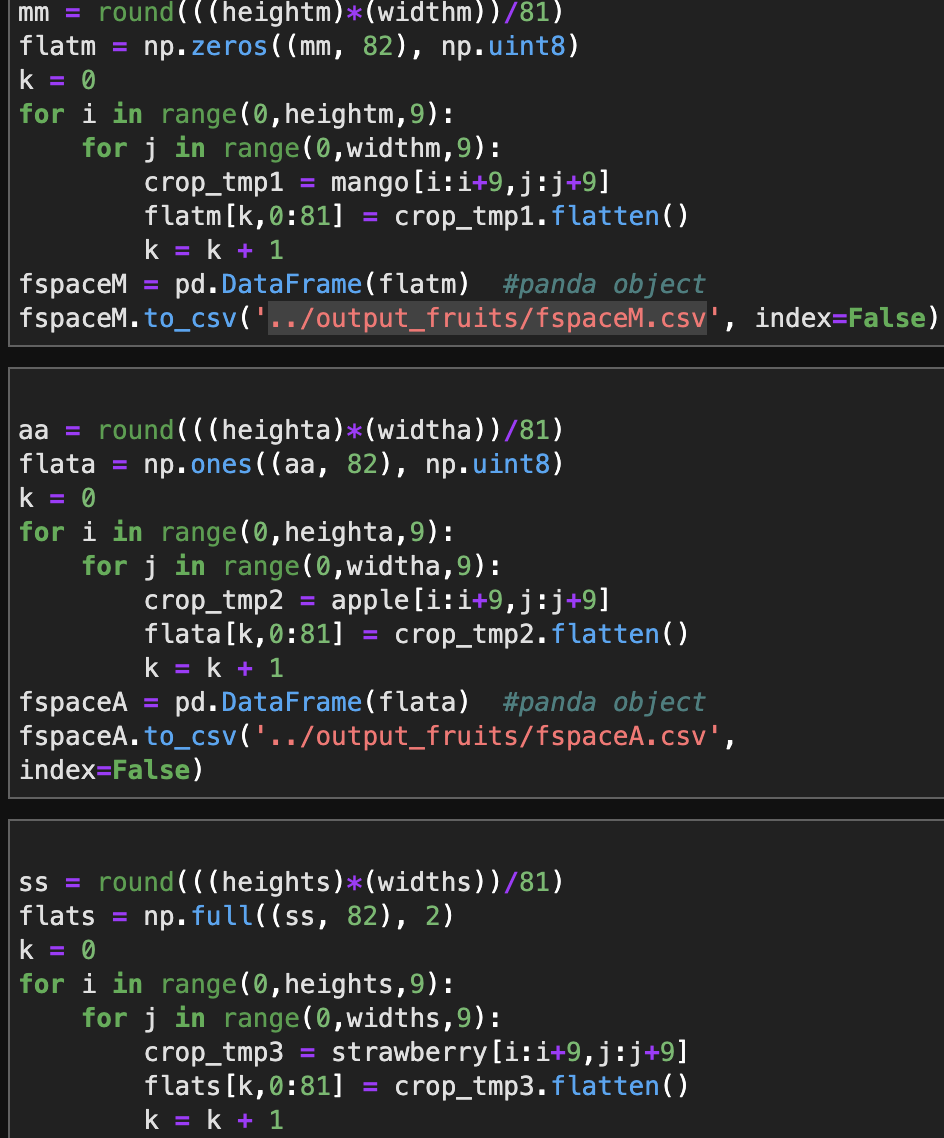
\includegraphics[height=9cm]{task6.png} 
    \caption{Task 5 }
  \label{fig:mangoGray-Resized }
    
\end{figure}

The generated spreadsheet for all three fruits is stored in the 'output_fruits' folder.\\
\begin{figure}[!htbp]
    \centering
    \includegraphics[height=6cm]{Task6.png} 
   
    \label{fig:my_label}
\end{figure}

\section{Task 7}
\subsection{Extract the statistical information from data}
We display the statistics like no of observations, minimum, maximum, dimension, mean and standard deviation. \\
We now get the mean and standard deviation of all the three fruits and represent them visually in the form of a line graph.

Apple Statistics: 
For Apple its selected feature have min value of 0 and max value of 255 and it mean is 111.72 and standard deviation is 59.95. The graph plotted for the features of Apple shows that $\textunderscore$ data increases from 0-1 of x-axis the standard deviation and mean remains contant and as the $\textunderscore$ decreases from 1-2 of x-axis the standard deviation and mean still remains constant.The output and graph for min,max,standard deviation,mean of Strawberry are shown in the graph above. \\
histogram: \\
\begin{figure}[!htbp]
    \centering
    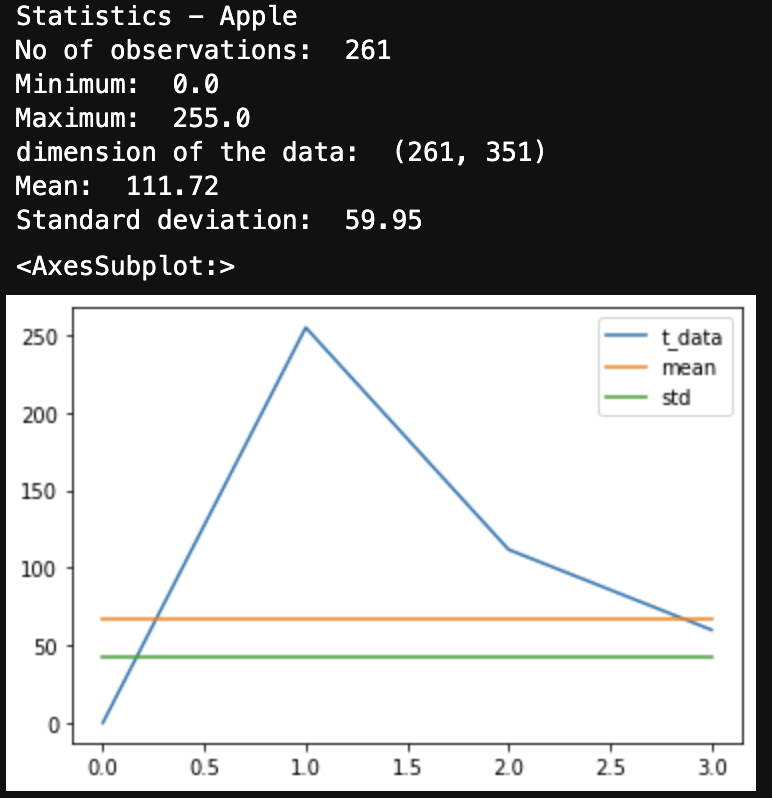
\includegraphics[height=3cm]{Task7_Apple.png} 
    \includegraphics[height=3cm]{Task2.35.png} 
    \label{fig:my_label}
\end{figure}

Mango Statistics \\
For Mango its selected feature have min value of 0 and max value of 255 and it mean is 156.32 and standard deviation is 45.73. The graph plotted for the features of mango shows that $\textunderscore$ data increases from 0-1 of x-axis the standard deviation and mean remains contant and as the $\textunderscore$ decreases from 1-2 of x-axis the standard deviation and mean still remains constant.The output and graph for min,max,standard deviation,mean of mango are shown in the graph above. \\
histogram: \\
\begin{figure}[!htbp]
    \centering
    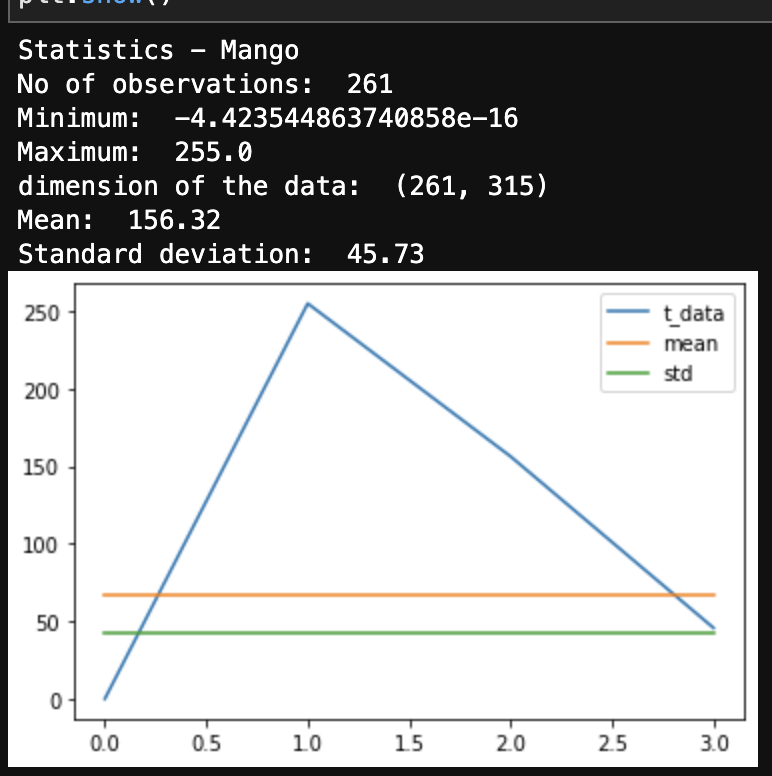
\includegraphics[height=3cm]{Task7_Mango.png} 
    \includegraphics[height=2cm,width=4cm]{Task2.36.png} 
    \label{fig:my_label}
\end{figure}

Strawberry Statistics \\
For Strawberry its selected feature have min value of 0 and max value of 255 aand it mean is 81.9 and standard deviation is 35.07. The graph plotted for the features of Strawberry shows that $\textunderscore$ data increases from 0-1 of x-axis the standard deviation and mean remains contant and as the $\textunderscore$ decreases from 1-2 of x-axis the standard deviation and mean still remains constant.The output and graph for min,max,standard deviation,mean of Strawberry are shown in the graph above.\\
histogram: \\
\begin{figure}[!htbp]
    \centering
    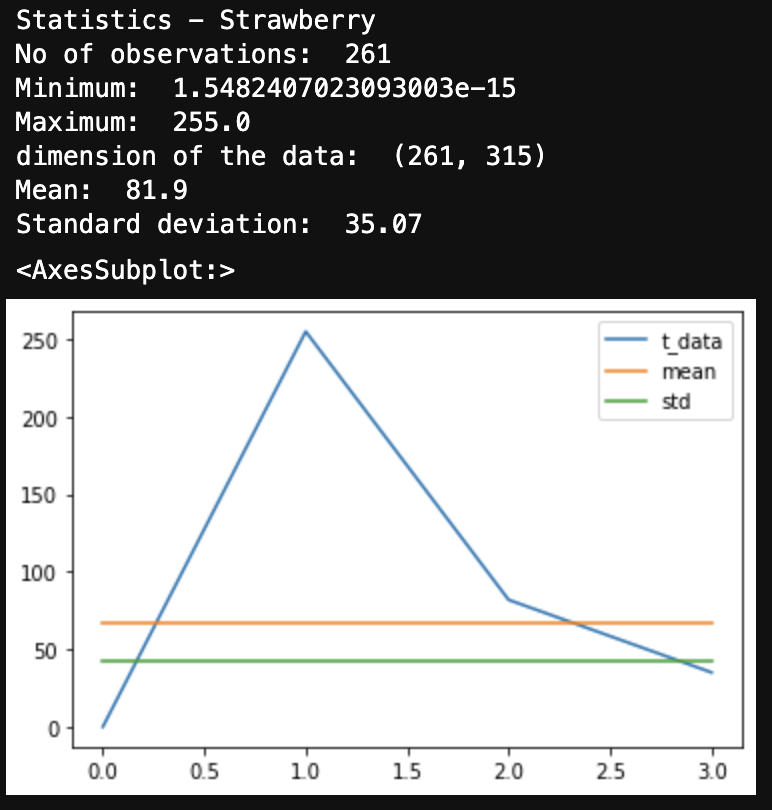
\includegraphics[height=3cm,width=4cm]{Task7_Strawberry.png} 
    \includegraphics[height=3cm,width=4cm]{Task2.37.png} 
    \label{fig:my_label}
\end{figure}
We plot the images as scatterplot by its color property as shown below, apple is shown by red color, mango by yellow and strawberry by pink. \\

\begin{figure}[!htbp]
    \centering
    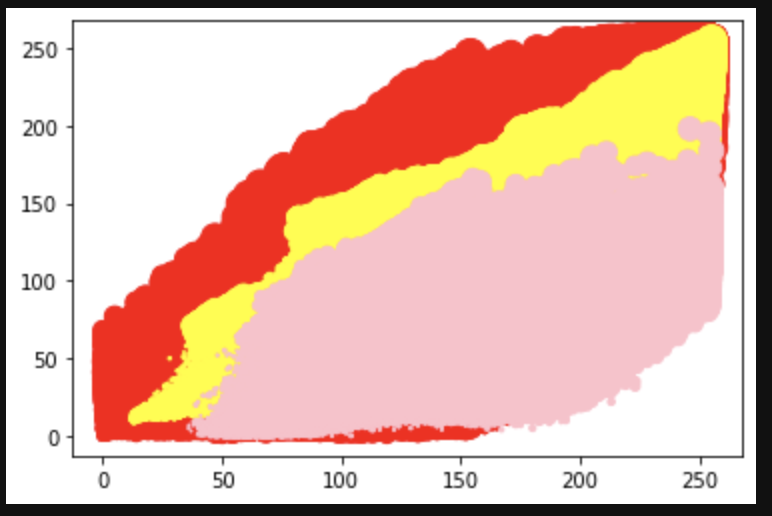
\includegraphics[height=4cm,width=4cm]{Task7-scatter.png} 
   
    \label{fig:my_label}
\end{figure}





\section{Task 8}
\subsection{Construct a feature space!}
To generate a feature space for these images, we first integrate the feature vectors in image0.csv and image1.csv. To build the suitable feature space for these image classes, each feature and label column aligns vertically. In the output folder, the created feature space is named 'image01.csv.'
\\ Similarly, we integrate the feature vectors in image0.csv, image1.csv, and image2.csv. To generate the suitable feature space for these three classes, each feature and label column must line vertically. The resulting feature space file is named 'image012.csv' and saved in the output folder.
In the files image01.csv and image012.csv, we now randomize the placement of the feature vectors. We don't randomize the content of a feature vector here, but the placement (rows) of the csv files. 
\begin{figure}[!htbp]
    \centering
    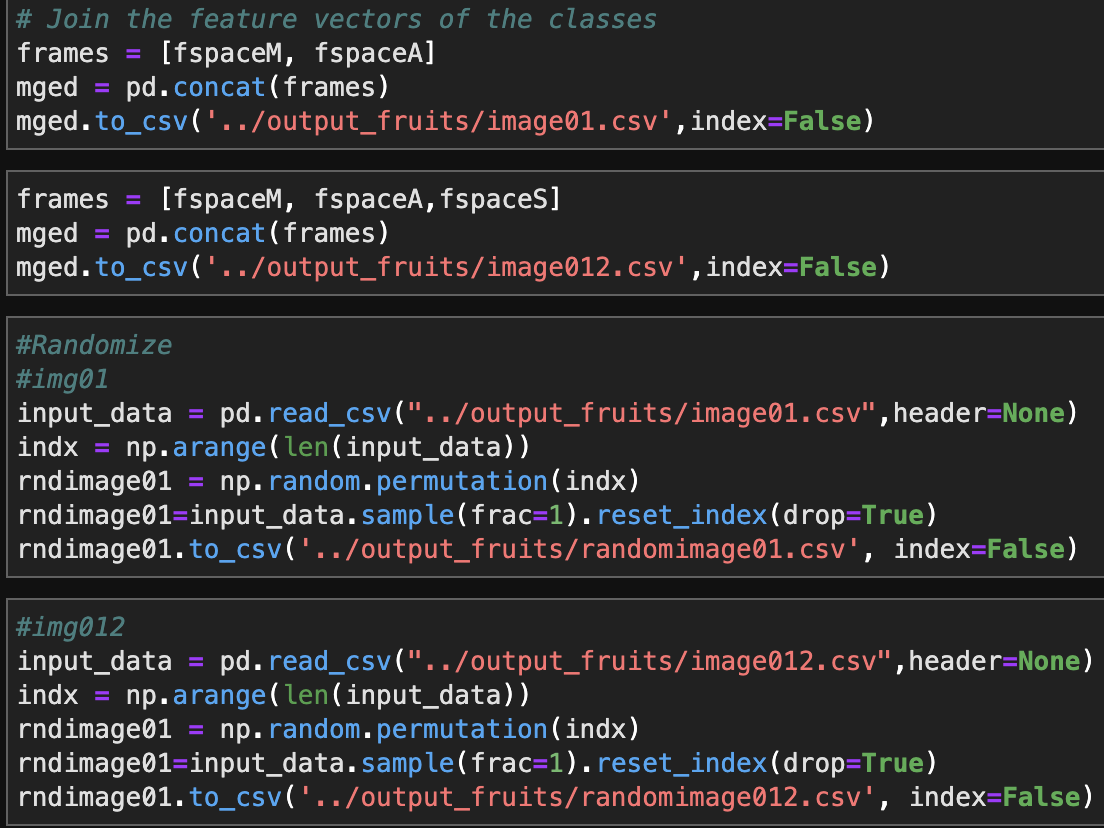
\includegraphics[height=6cm]{Task8.png} 
   
    \label{fig:my_label}
\end{figure}
\\Finally, we randomize the generated image01.csv and image012.csv file and generate two new files randomimage01.csv and randomimage012.csv respectively.\\
\section{Task 9}
\subsection{Display subspaces!}
Using the spreadsheets that we prepared, we select two features and plot the two-dimensional feature space, labeling the observations (vectors) of the fruits or vegetables that we selected. To plot a two-dimensional feature space, we use the Apple and mango spreadsheet to choose the fruits.
\begin{figure}[!htbp]
    \centering
    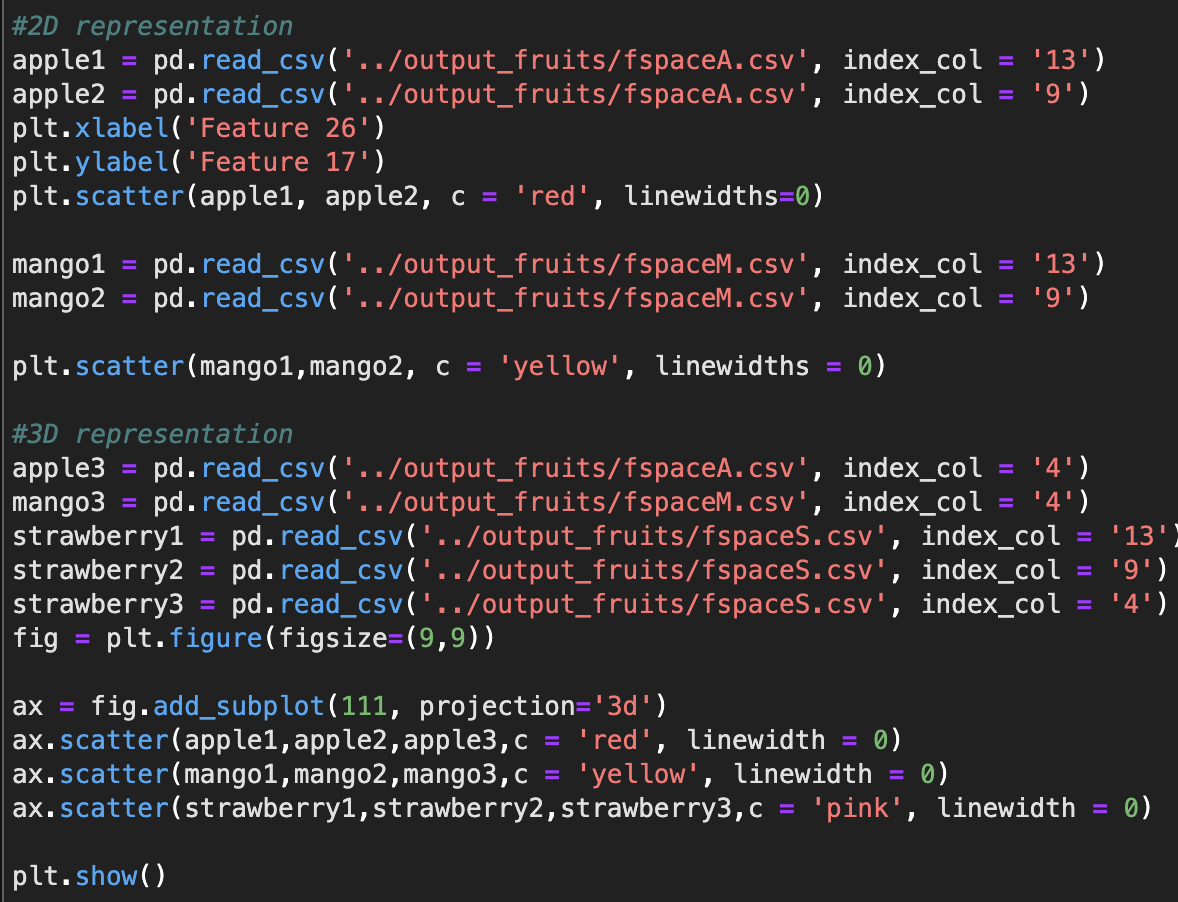
\includegraphics[height=6cm]{Task9.png} 
   
    \label{fig:my_label}
\end{figure}
\begin{figure}[!htbp]
    \centering
    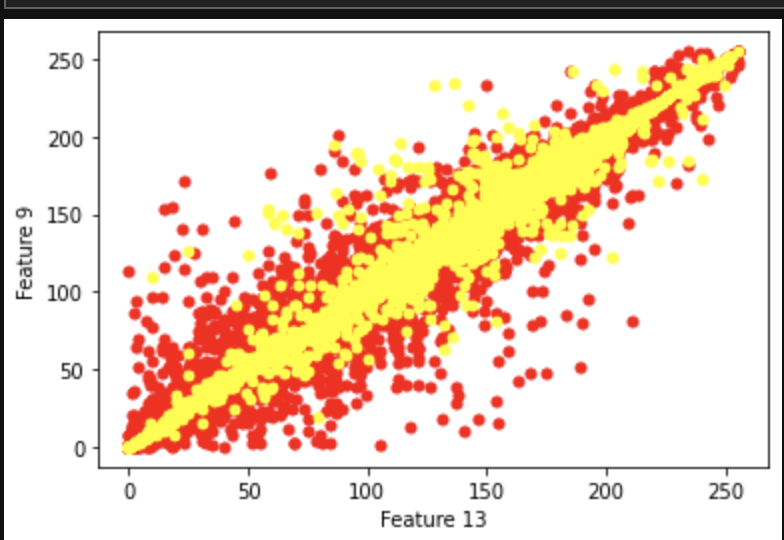
\includegraphics[height=4cm]{Task9-2d(1).png} 
   
    \label{fig:my_label}
\end{figure}
\\From the above graph we see various points in which our features are spread out.
\\\\
Then, using the spreadsheets we created, we select three features and plot the three-dimensional feature space, labeling the observations (vectors) of the fruits or vegetables we chose. Feature 26, Feature 17, and Feature 4 of our fruits Apple, Mango, and Strawberry are now plotted.
\begin{figure}[!htbp]
    \centering
    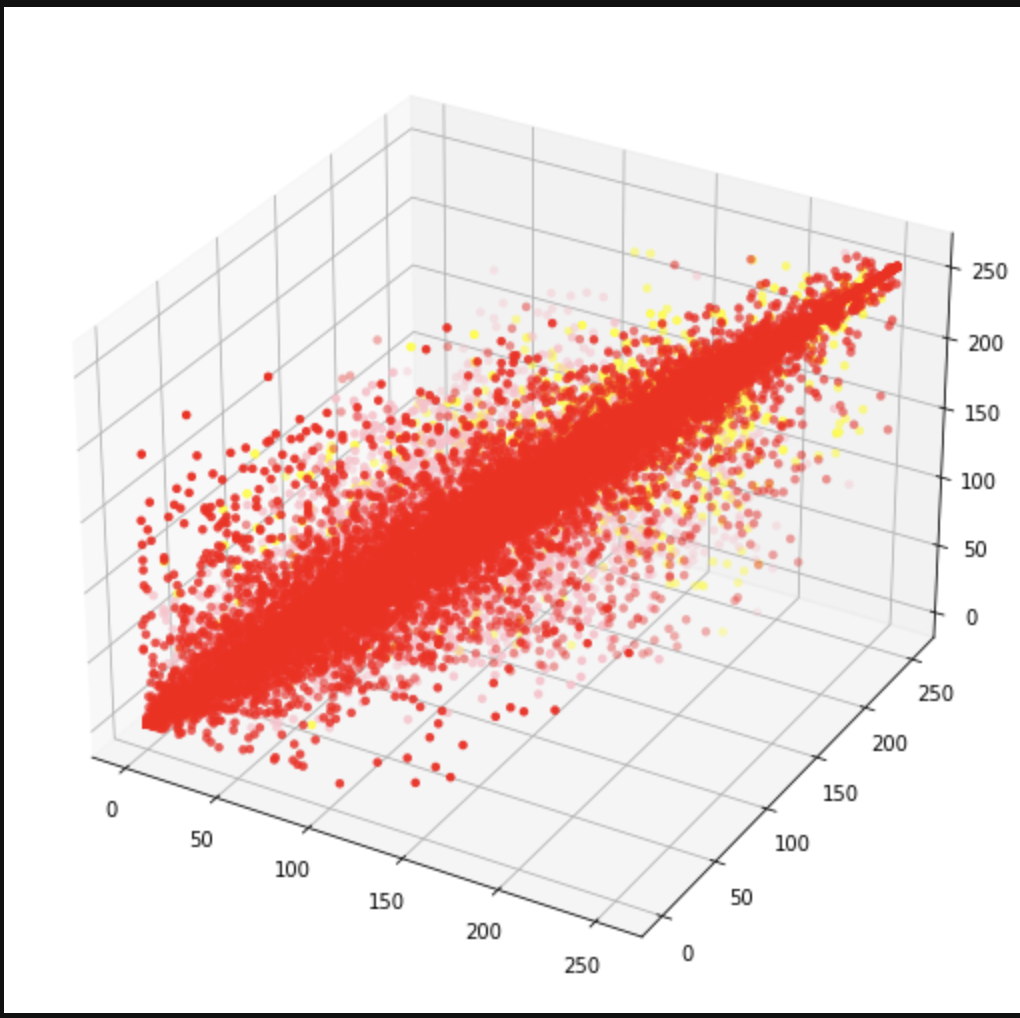
\includegraphics[height=4cm]{Task9-3d.png} 
   
    \label{fig:my_label}
\end{figure}
\\From the graph above, we can see the various distinct plotted points of each feature of all the fruits. \\

\section{Task 10 - converting all the images in a folder}
Now we'll construct Python code to read any number of images from a folder of many similar images, create feature spaces, and create spreadsheets for the feature spaces.
\begin{figure}[!htbp]
    \centering
    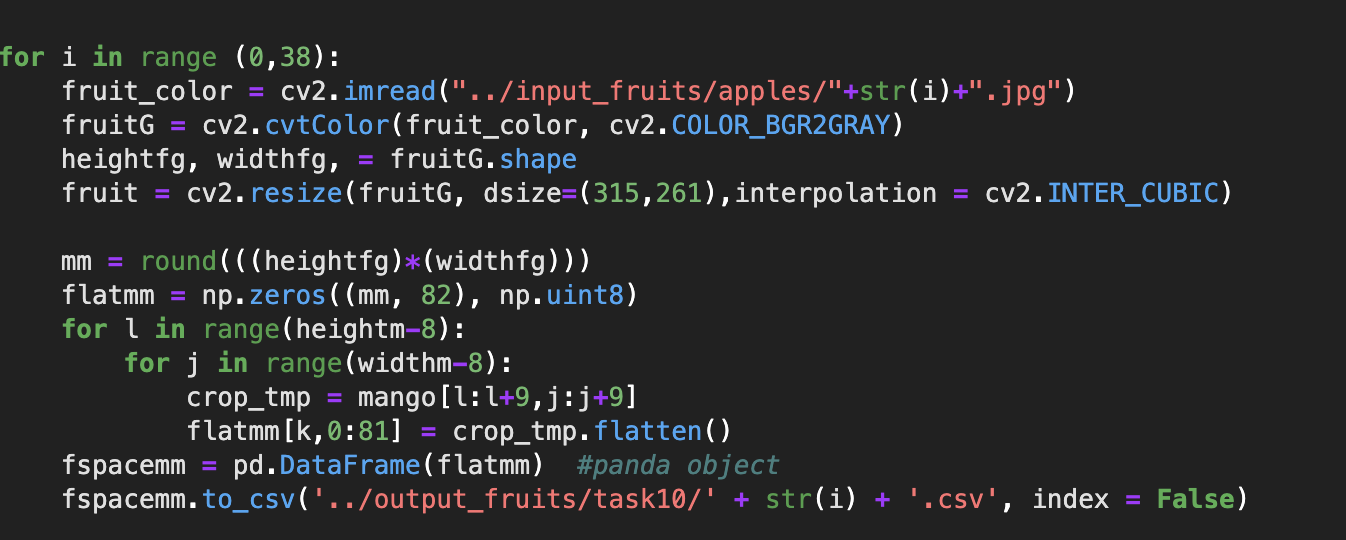
\includegraphics[height=6cm]{task10-code.png} 
   
    \label{fig:my_label}
\end{figure}
\\\\In this code we try to read all the images under the folder '$input fruits->apples$'. The generated spreadsheets for the images under this folder are stored under 'Task 10' in the output folder.
\begin{figure}[!htbp]
    \centering
    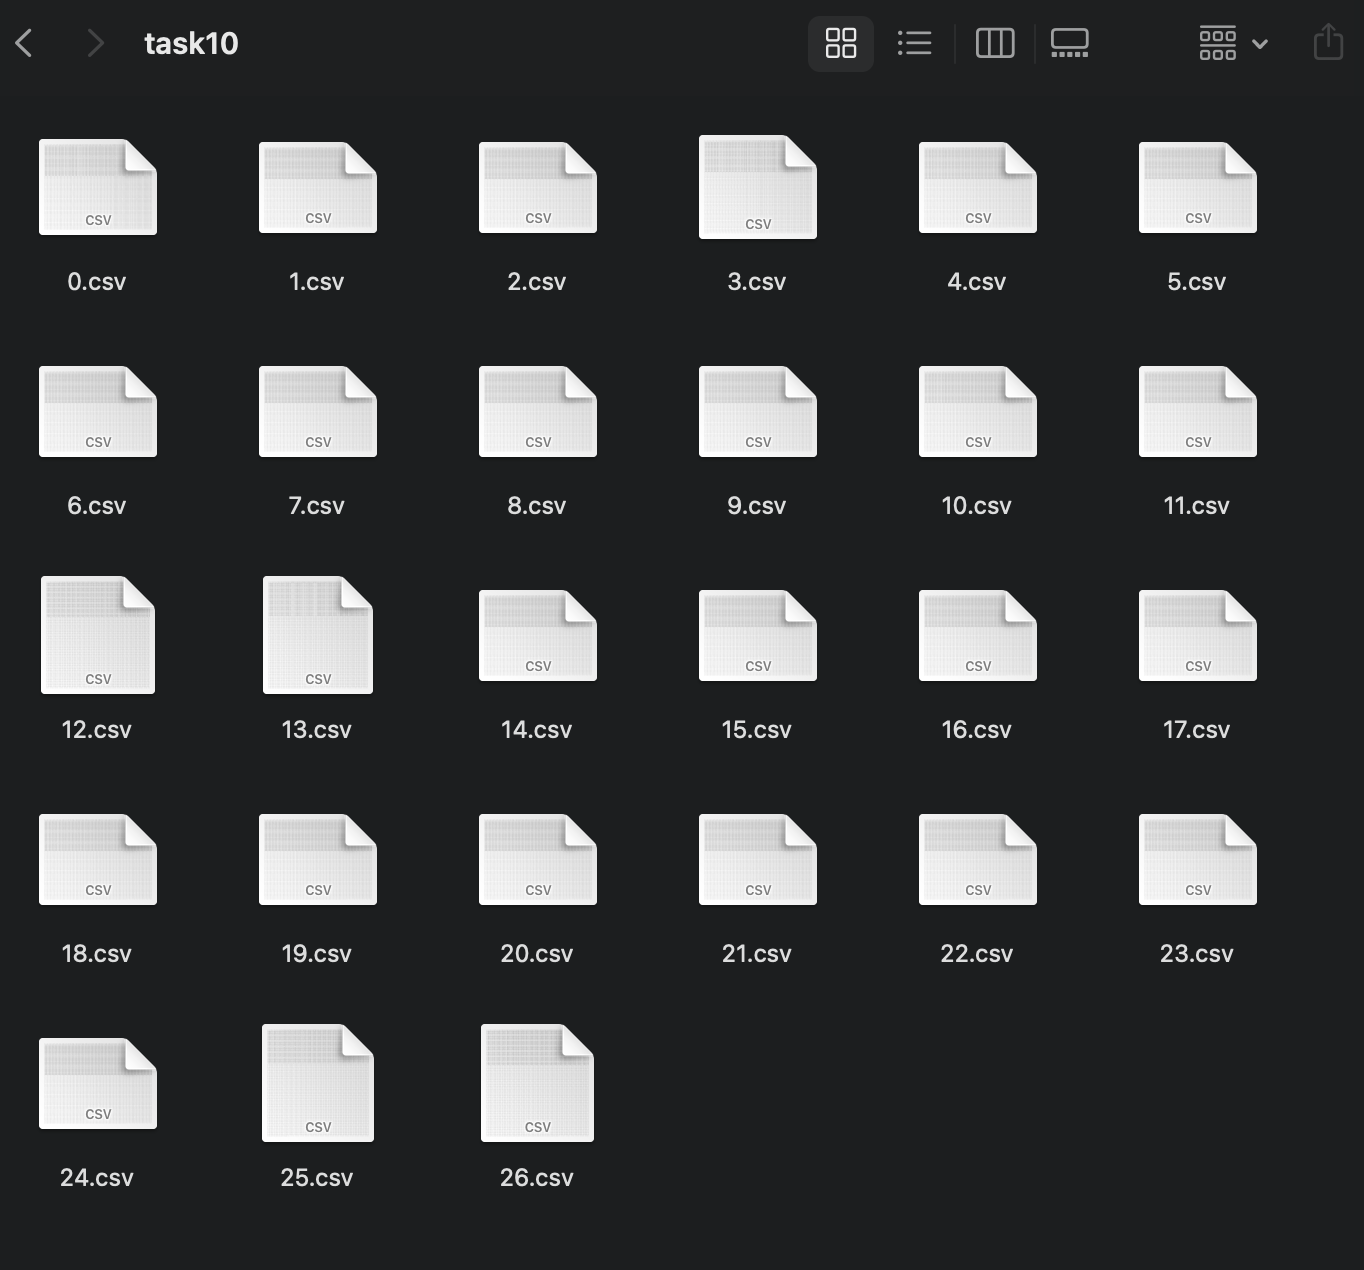
\includegraphics[height=3cm]{output.png} 
   
    \label{fig:my_label}
\end{figure}
As you can see, outputs are generated under '$output fruits/task10$' for all the images in the input folder.

\section{Task 11}

We move into higher dimensions when we have a larger block size. Our data becomes increasingly sparse and evenly spread in higher dimensions. As a result, the classifier has a hard time distinguishing between the features and learning from them. As a result, we minimize the block size to assist our classifier in training models more efficiently and quickly.\\
\pagebreak
\maketitle
\section{Assignment 02: Feature Space to a Classifier}
\section{TASK 1 }
\subsection{Complete and extend the tasks of assignment 1}
The four categories of datasets created in the first stage are
\begin{enumerate}
\item
Non overlapping 2 class 
\item
Non overlapping multi class
\item
Overlapping 2 class
\item
Overlapping multi class
\end{enumerate}
we are reading all these categories datasets which are saved in the Assignment 1.
\begin{figure}[!htbp]
    \centering
    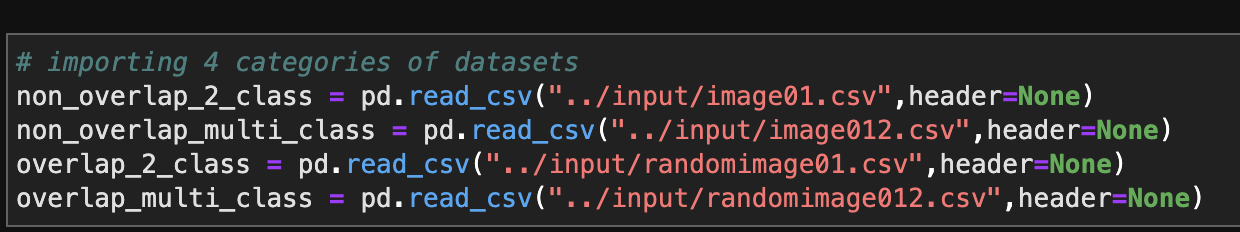
\includegraphics[height=1.7cm]{task1.1.png} 
   
    \label{fig:my_label}
\end{figure}
\subsection{Divide the data domain of the data sets into training and testing sets}
All the four categories of data are split into training and testing sets of ratio 78:22 respectively,
Below example is the shape of non overlapping 2 class classification after the split.
\begin{figure}[!htbp]
    \centering
    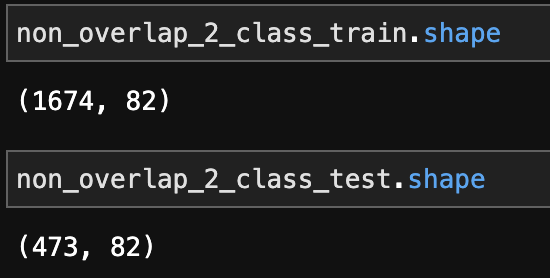
\includegraphics[height=3cm]{task1.2.png} 
   
    \label{fig:my_label}
\end{figure}
\subsection{Selecting features and plotting their Histograms and Scatter Plots}
Feature Selection: \\
Two features 13 and 26 are selected in training and testing sets of every category as follows.
\begin{figure}[!htbp]
    \centering
    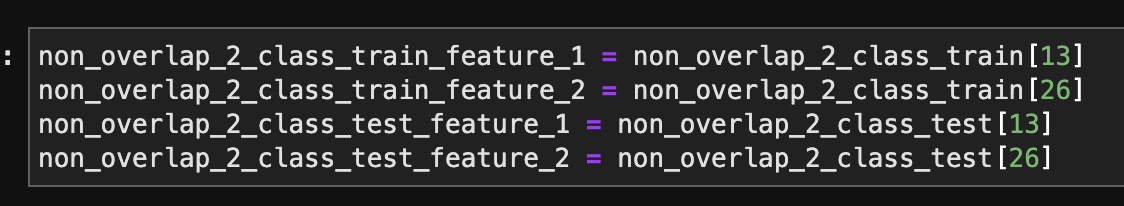
\includegraphics[height=1.7cm]{task1.3.png} 
   
    \label{fig:my_label}
\end{figure}
Histograms: \\
Histograms of each category and two datasets in each category are plotted.The histograms of two features are plotted in an overlapping manner to show whether they follow a similar distribution or not. \\
The following are the histograms and their statistics like mean and variance.
\begin{figure}
    \centering
    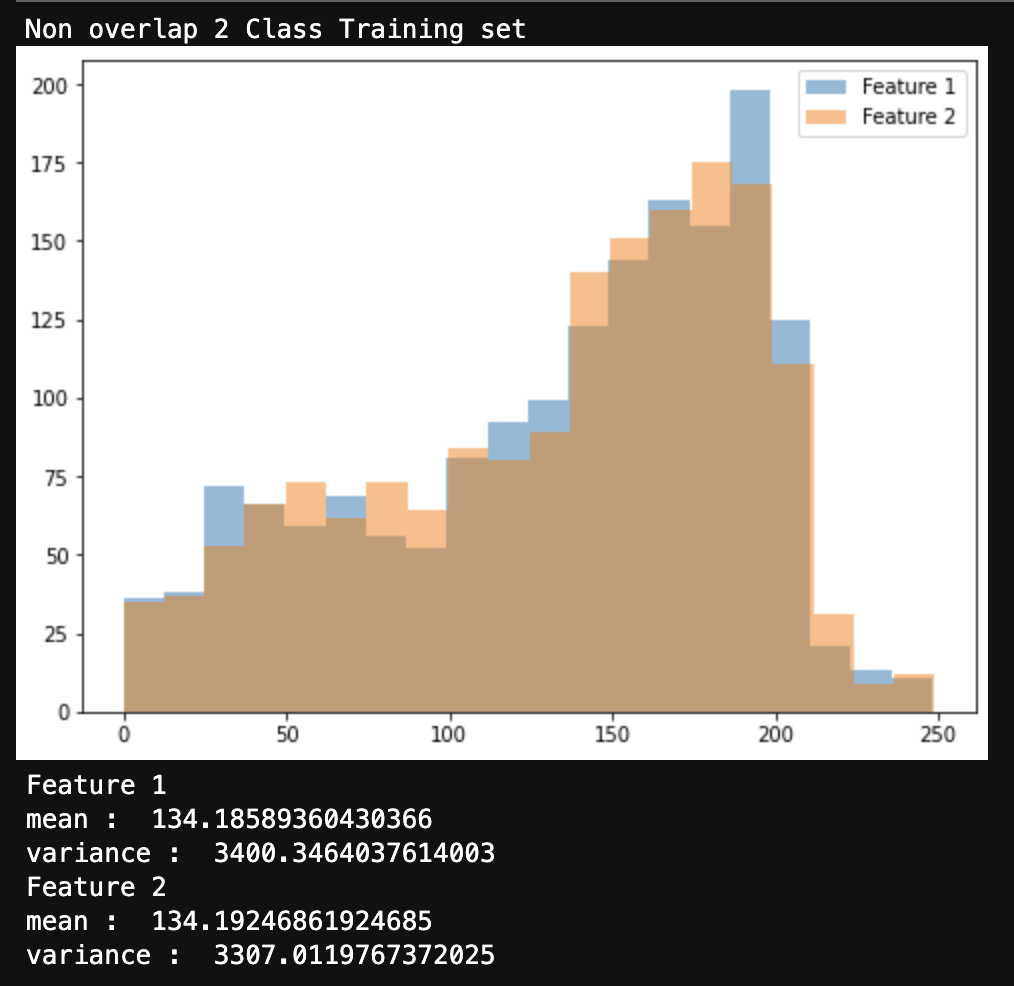
\includegraphics[width=5cm, height=6cm]{task1.5.png} 
    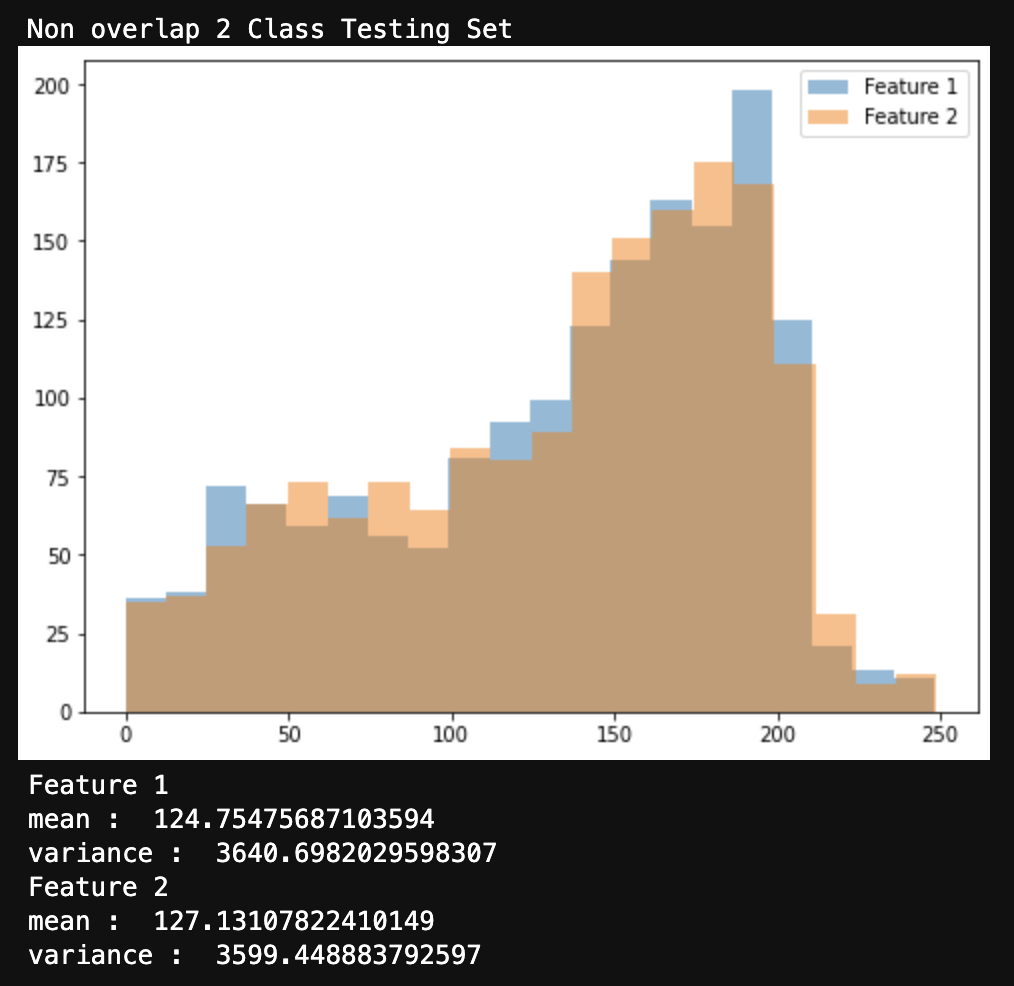
\includegraphics[width=5cm, height=6cm]{task1.6.png}
    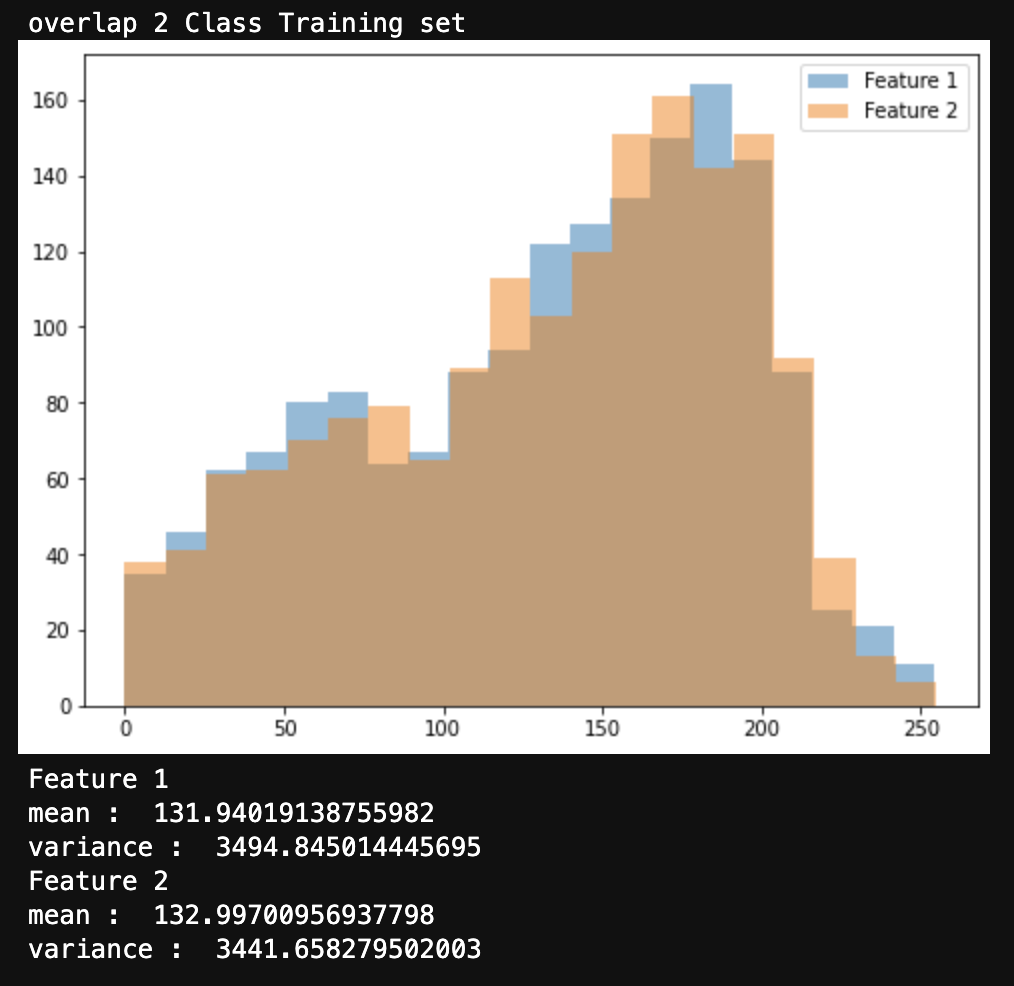
\includegraphics[width=5cm, height=6cm]{task1.7.png}
    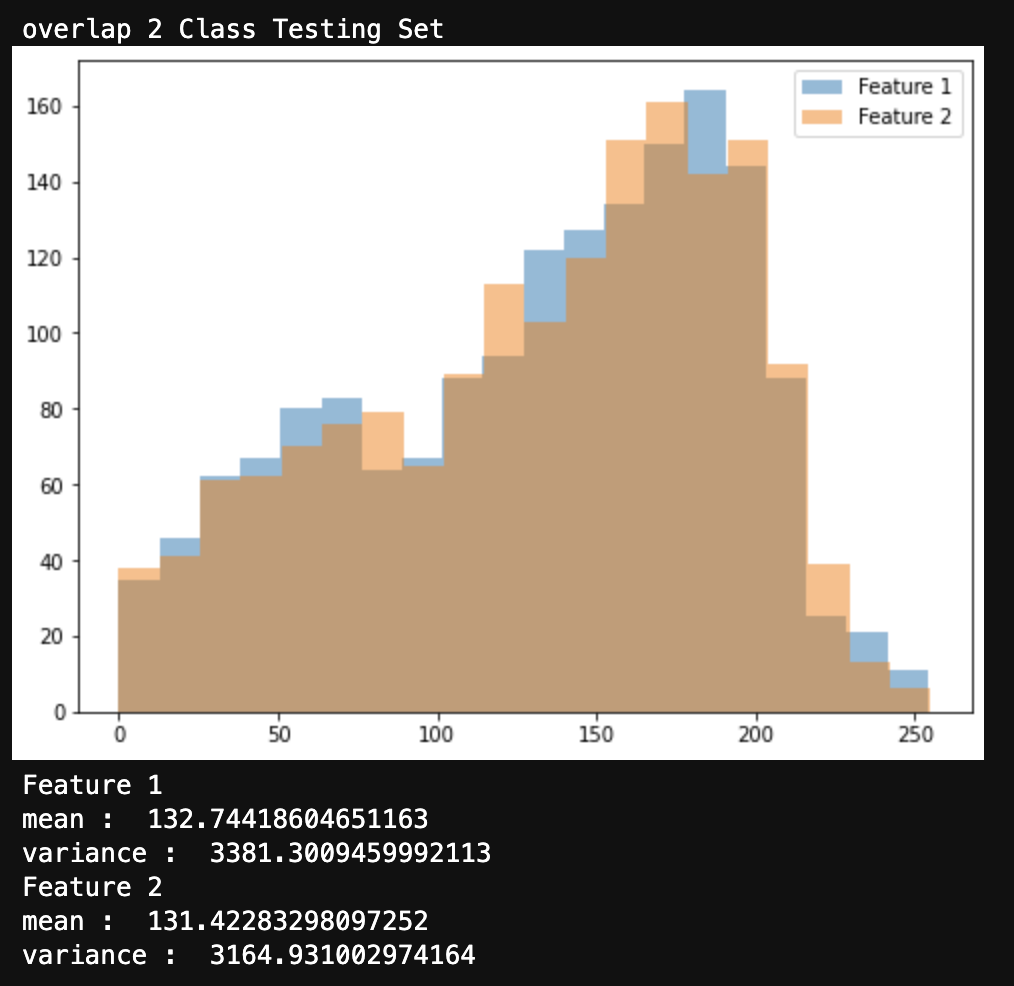
\includegraphics[width=5cm, height=6cm]{task1.8.png}
    \label{fig:my_label}
\end{figure}
\pagebreak
\begin{figure}
    \centering
    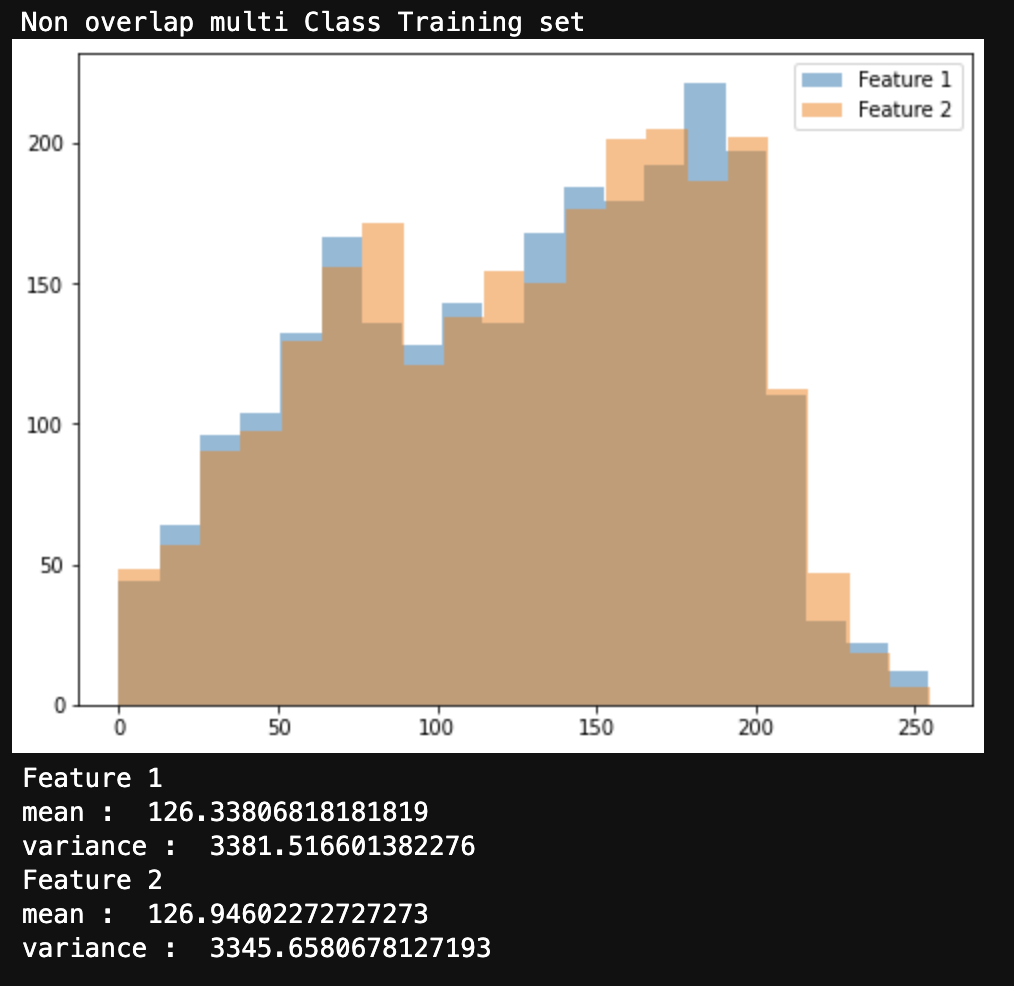
\includegraphics[width=5cm, height=4cm]{task1.9.png} 
    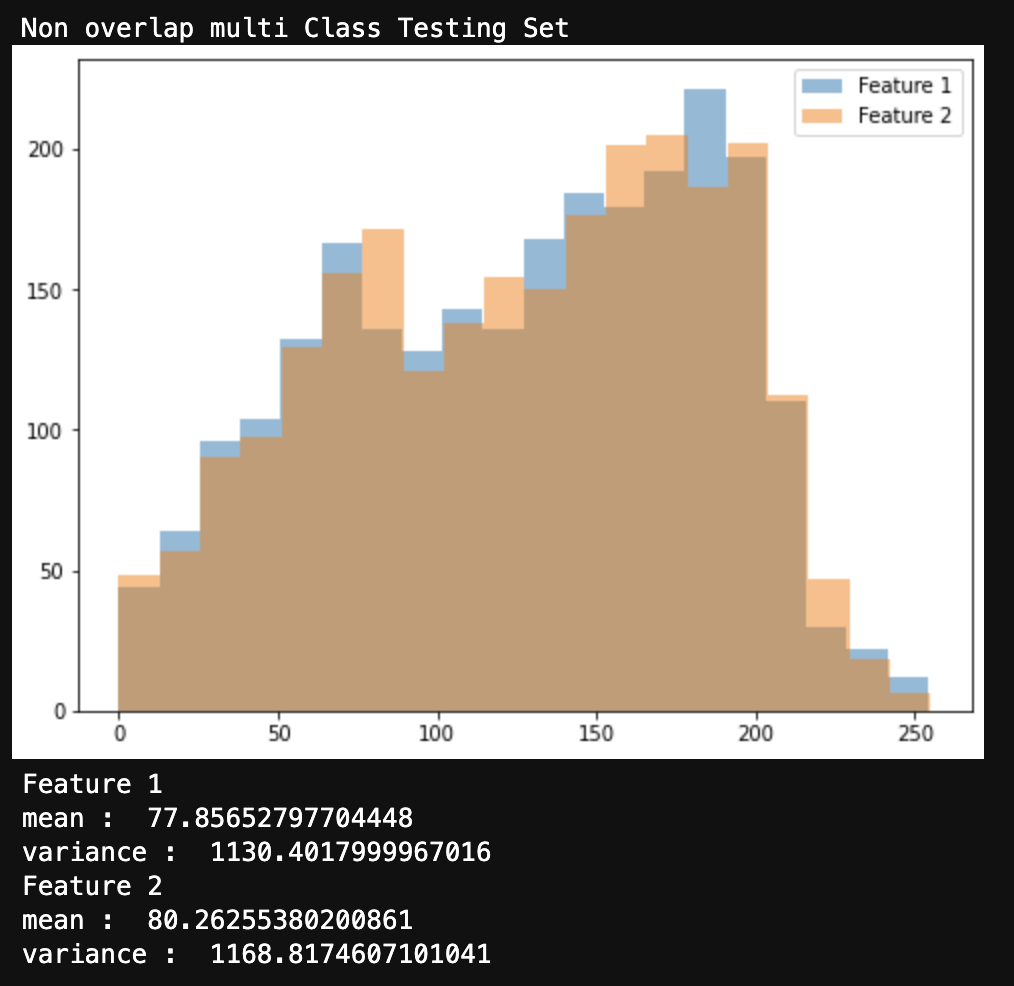
\includegraphics[width=5cm, height=4cm]{task1.10.png}
    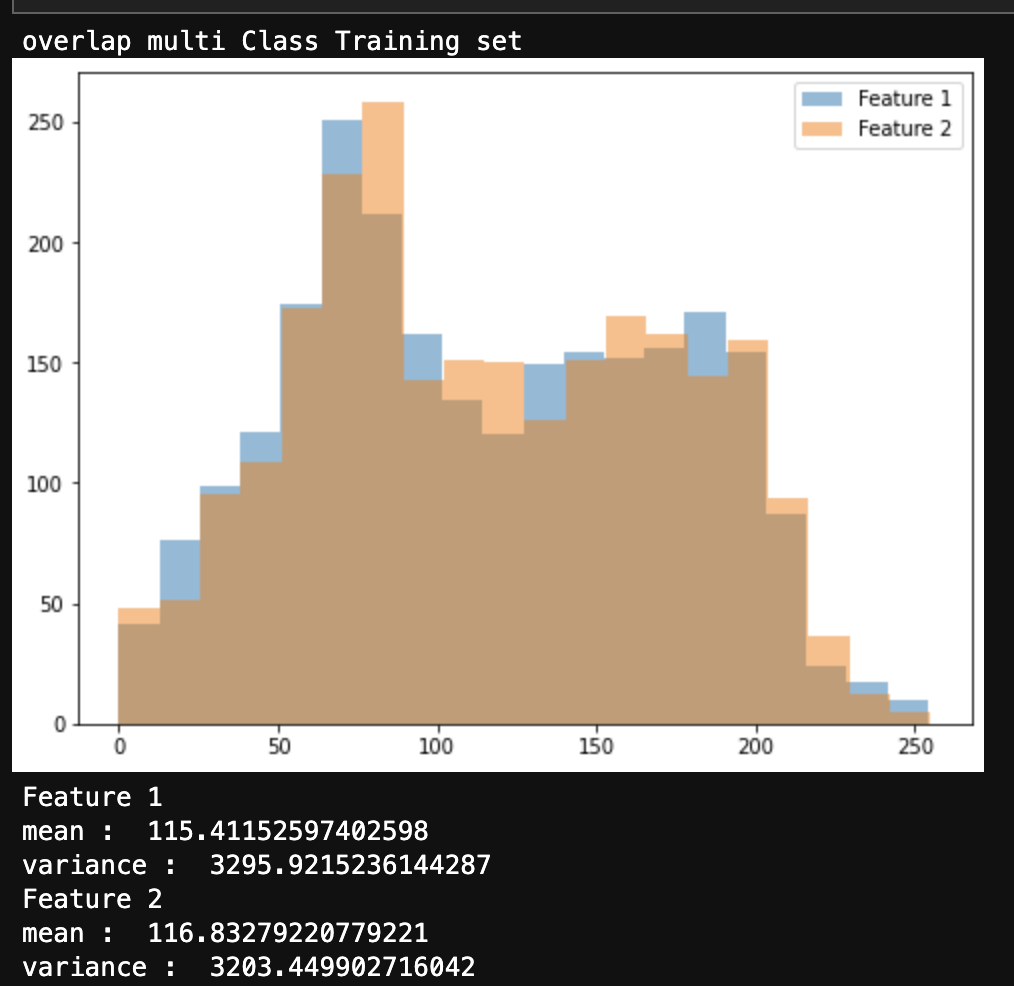
\includegraphics[width=5cm, height=4cm]{task1.11.png}
    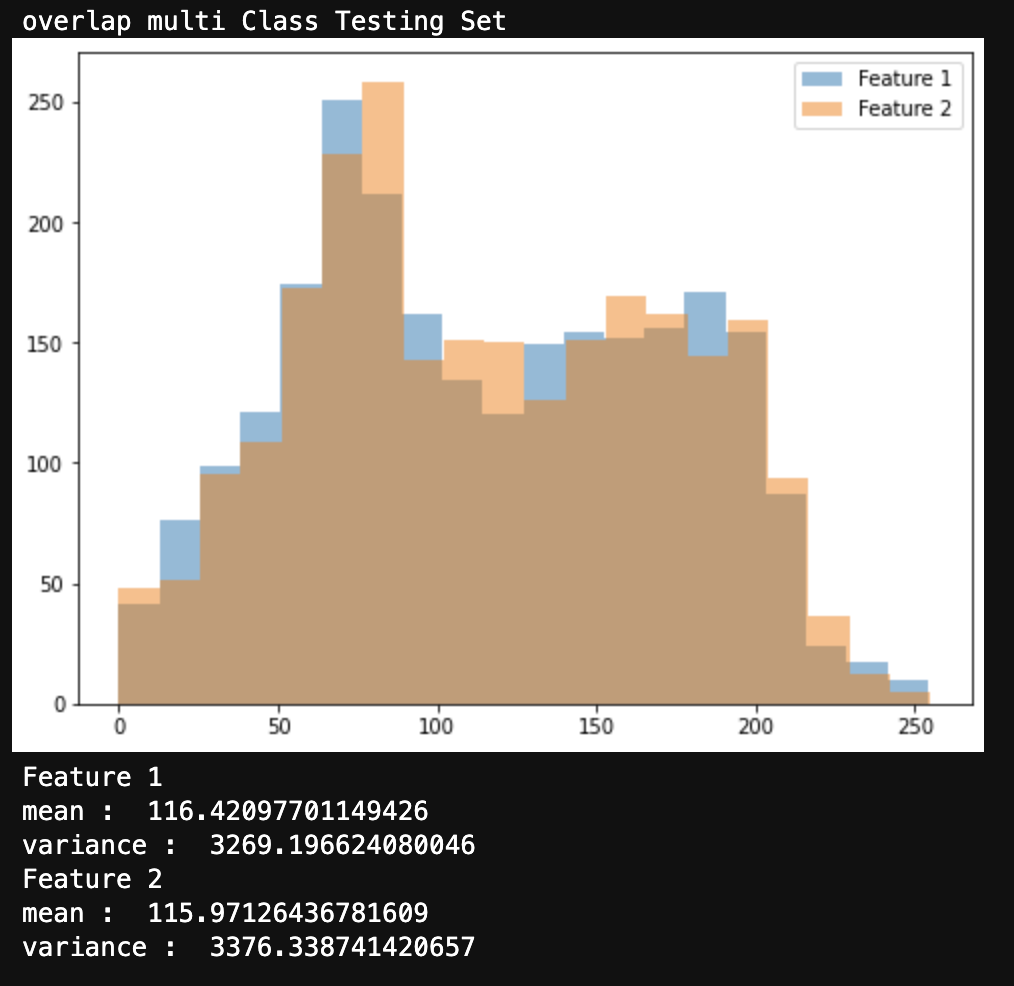
\includegraphics[width=5cm, height=4cm]{task1.12.png}
    \label{fig:my_label}
\end{figure} 
In all these histograms, we can observe that the statistics and distribution of two features in a dataset is almost the same To further investigate this point, let us plot scatter plots for all the features.
\begin{figure}
    \centering
    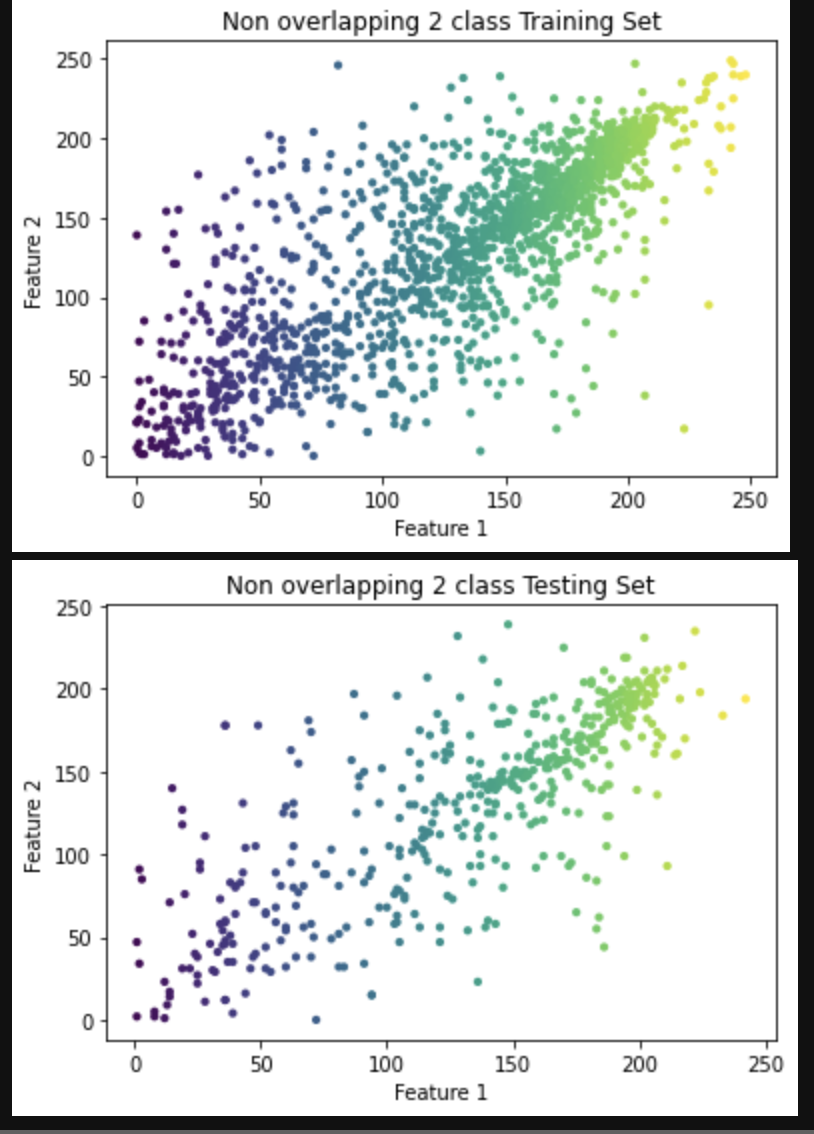
\includegraphics[width=5cm, height=6cm]{task1.13.png} 
    \includegraphics[width=5cm, height=6cm]{task1.14.png}
    \includegraphics[width=5cm, height=6cm]{task1.15.png}
    \includegraphics[width=5cm, height=6cm]{task1.16.png}
    \label{fig:my_label}
\end{figure}
In these scatter plots, despite a few outliers, the data follows a linear fashion, which means that the features are almost similar.
\pagebreak
\section{TASK 2 }
\subsection{Implementing lasso regression and add predicted label column to respective test dataset}
Lasso regression is implemented and used as a two class classifier to classify overlapped and non-overlapped 2 class datasets. Although it is mentioned to use lasso regression as 2 class classifier only in the subtask 1, in the subtask 2 it is written to test the test sets of all the categories of datasets, so I assumed that multi class classifier should also be created. Hence I have used lasso regression to create both two class and multi class classifier and classified all the 4 categories of data. \\
\textbf{Training the model and Testing the results:}\\
\begin{enumerate}
\item
Non overlapping 2 class: \\
for the non overlapping two class, Training set is split into X\_train (containing all the features) and y\_train (actual labels) and the model is trained as shown below.
\begin{figure}[!htbp]
    \centering
    \includegraphics[width=8cm, height=2cm]{task2.1.png}
    \label{fig:my_label}
\end{figure}
In the same way, the model is tested on test set and the predicted results are added in an additional column as shown below.
\begin{figure}[!htbp]
    \centering
    \includegraphics[width=5cm, height=5cm]{task2.2.png}
    \label{fig:my_label}
\end{figure}
\item
Non overlapping multi class: \\
for the non overlapping multi class, Training set is split into X\_train (containing all the features) and y\_train (actual labels) and the model is trained as shown below.
\begin{figure}[!htbp]
    \centering
    \includegraphics[width=8cm, height=2cm]{task2.3.png}
    \label{fig:my_label}
\end{figure}
In the same way, the model is tested on test set and the predicted results are added in an additional column as shown below.
\begin{figure}[!htbp]
    \centering
    \includegraphics[width=5cm, height=5cm]{task2.4.png}
    \label{fig:my_label}
\end{figure}
\item
Overlapping 2 class \\
for the overlapping 2 class, Training set is split into X\_train (containing all the features) and y\_train (actual labels) and the model is trained as shown below.
\begin{figure}[!htbp]
    \centering
    \includegraphics[width=8cm, height=2cm]{task2.5.png}
    \label{fig:my_label}
\end{figure}
In the same way, the model is tested on test set and the predicted results are added in an additional column as shown below.
\begin{figure}[!htbp]
    \centering
    \includegraphics[width=5cm, height=5cm]{task2.6.png}
    \label{fig:my_label}
\end{figure}
\item
Overlapping multi class \\
or the overlapping multi class, Training set is split into X\_train (containing all the features) and y\_train (actual labels) and the model is trained as shown below.
\begin{figure}[!htbp]
    \centering
    \includegraphics[width=8cm, height=2cm]{task2.7.png}
    \label{fig:my_label}
\end{figure}
In the same way, the model is tested on test set and the predicted results are added in an additional column as shown below.
\begin{figure}[!htbp]
    \centering
    \includegraphics[width=5cm, height=5cm]{task2.8.png}
    \label{fig:my_label}
\end{figure}
\end{enumerate}
\subsection{Construct Confusion matrix for each category}
\begin{enumerate}
\item
Non overlapping 2 class: \\
Below is the confusion matrix \\
\begin{figure}[!htbp]
    \centering
    \includegraphics[width=4cm, height=4cm]{task2.9.png}
    \label{fig:my_label}
\end{figure}
We can see that our model is poorly trained, this is because the data in the training set is imbalanced, the ratio of the class labels is not equal. This can be understood by looking at the below value counts. \\
\begin{figure}[!htbp]
    \centering
    \includegraphics[width=4cm, height=2cm]{task2.13.png}
    \label{fig:my_label}
\end{figure}
\item
Non overlapping multi class: \\
Below is the confusion matrix \\
\begin{figure}[!htbp]
    \centering
    \includegraphics[width=4cm, height=4cm]{task2.10.png}
    \label{fig:my_label}
\end{figure}
We can see that our model is poorly trained, this is because the data in the training set is imbalanced, the ratio of the class labels is not equal. This can be understood by looking at the below value counts. \\
\begin{figure}[!htbp]
    \centering
    \includegraphics[width=4cm, height=2cm]{task2.14.png}
    \label{fig:my_label}
\end{figure}
\item
overlapping 2 class: \\
Below is the confusion matrix \\
\begin{figure}[!htbp]
    \centering
    \includegraphics[width=4cm, height=4cm]{task2.11.png}
    \label{fig:my_label}
\end{figure}
We can see that our model is properly trained, this is because the data in the training set is balanced, the ratio of the class labels is almost equal. This can be understood by looking at the below value counts. \\
\begin{figure}[!htbp]
    \centering
    \includegraphics[width=4cm, height=2cm]{task2.15.png}
    \label{fig:my_label}
\end{figure}
\item
overlapping multi class: \\
Below is the confusion matrix \\
\begin{figure}[!htbp]
    \centering
    \includegraphics[width=3cm, height=3cm]{task2.12.png}
    \label{fig:my_label}
\end{figure}
We can see that our model is properly trained, this is because the data in the training set is balanced, the ratio of the class labels is almost equal. This can be understood by looking at the below value counts. \\
\begin{figure}[!htbp]
    \centering
    \includegraphics[width=4cm, height=1.5cm]{task2.16.png}
    \label{fig:my_label}
\end{figure}
\end{enumerate}

\subsection{Qualitative measures - Confusion Matrix based}
Specificity and Sensitivity are chosen as the confusion based qualitative measures for this task. \\
Specificity is calculated by TN/TN+FP \\
Sensitivity is calculated by TP/TP+FN \\
But when it comes to multi class classification, both these measures are individually calculated and their average is considered as final quality measure. \\
All these values are calculated from the confusion matrix and measured. Below are the values of each category. \\
\begin{enumerate}
    \item 
    Non overlapping 2 class: \\
Below are the values \\
\begin{figure}[!htbp]
    \centering
    \includegraphics[width=6cm, height=2cm]{task2.27.png}
    \label{fig:my_label}
\end{figure}
\item
Non overlapping multi class: \\
Below are the values \\
\begin{figure}[!htbp]
    \centering
    \includegraphics[width=6cm, height=2cm]{task2.28.png}
    \label{fig:my_label}
\end{figure}
\item
overlapping 2 class: \\
Below are the values \\
\begin{figure}[!htbp]
    \centering
    \includegraphics[width=6cm, height=2cm]{task2.29.png}
    \label{fig:my_label}
\end{figure}
\item
overlapping multi class: \\
Below are the values \\
\begin{figure}[!htbp]
    \centering
    \includegraphics[width=6cm, height=2cm]{task2.30.png}
    \label{fig:my_label}
\end{figure}
    

\end{enumerate}
\section{TASK 3 }
\subsection{Implementing random forest and add predicted label column to respective test dataset}
Random Forest is implemented and used as a two class classifier and multi class classifier to classify all the 4 categories of data. \\
\textbf{Training the model and Testing the results:}\\
\begin{enumerate}
\item
Non overlapping 2 class: \\
for the non overlapping two class, Training set is split into X\_train (containing all the features) and y\_train (actual labels) and the model is trained as shown below.
\begin{figure}[!htbp]
    \centering
    \includegraphics[width=8cm, height=2cm]{task2.17.png}
    \label{fig:my_label}
\end{figure}
In the same way, the model is tested on test set and the predicted results are added in an additional column.
\item
Non overlapping multi class: \\
for the non overlapping multi class, Training set is split into X\_train (containing all the features) and y\_train (actual labels) and the model is trained as shown below.
\begin{figure}[!htbp]
    \centering
    \includegraphics[width=8cm, height=2cm]{task2.18.png}
    \label{fig:my_label}
\end{figure}
In the same way, the model is tested on test set and the predicted results are added in an additional column.
\item
Overlapping 2 class \\
for the overlapping 2 class, Training set is split into X\_train (containing all the features) and y\_train (actual labels) and the model is trained as shown below.
\begin{figure}[!htbp]
    \centering
    \includegraphics[width=8cm, height=2cm]{task2.19.png}
    \label{fig:my_label}
\end{figure}
In the same way, the model is tested on test set and the predicted results are added in an additional column.
\item
Overlapping multi class \\
or the overlapping multi class, Training set is split into X\_train (containing all the features) and y\_train (actual labels) and the model is trained as shown below.
\begin{figure}[!htbp]
    \centering
    \includegraphics[width=8cm, height=2cm]{task2.20.png}
    \label{fig:my_label}
\end{figure}
In the same way, the model is tested on test set and the predicted results are added in an additional column.
\end{enumerate}
\subsection{Construct Confusion matrix for each category}
\begin{enumerate}
\item
Non overlapping 2 class: \\
Below is the confusion matrix \\
\begin{figure}[!htbp]
    \centering
    \includegraphics[width=4cm, height=4cm]{task2.21.png}
    \label{fig:my_label}
\end{figure}
\item
Non overlapping multi class: \\
Below is the confusion matrix \\
\begin{figure}[!htbp]
    \centering
    \includegraphics[width=4cm, height=4cm]{task2.22.png}
    \label{fig:my_label}
\end{figure}
\item
overlapping 2 class: \\
Below is the confusion matrix \\
\begin{figure}[!htbp]
    \centering
    \includegraphics[width=3cm, height=3cm]{task2.23.png}
    \label{fig:my_label}
\end{figure}
\item
overlapping multi class: \\
Below is the confusion matrix \\
\begin{figure}[!htbp]
    \centering
    \includegraphics[width=3cm, height=3cm]{task2.24.png}
    \label{fig:my_label}
\end{figure}
\end{enumerate}
\subsection{Qualitative measures - Confusion Matrix based}
Specificity and Sensitivity are chosen as the confusion based qualitative measures for this task. \\
Specificity is calculated by TN/TN+FP \\
Sensitivity is calculated by TP/TP+FN \\
But when it comes to multi class classification, both these measures are individually calculated and their average is considered as final quality measure. \\
All these values are calculated from the confusion matrix and measured. Below are the values of each category. \\
\begin{enumerate}
    \item 
    Non overlapping 2 class: \\
Below are the values \\
\begin{figure}[!htbp]
    \centering
    \includegraphics[width=6cm, height=2cm]{task2.31.png}
    \label{fig:my_label}
\end{figure}
\item
Non overlapping multi class: \\
Below are the values \\
\begin{figure}[!htbp]
    \centering
    \includegraphics[width=6cm, height=2cm]{task2.32.png}
    \label{fig:my_label}
\end{figure}
\item
overlapping 2 class: \\
Below are the values \\
\begin{figure}[!htbp]
    \centering
    \includegraphics[width=6cm, height=2cm]{task2.33.png}
    \label{fig:my_label}
\end{figure}
\item
overlapping multi class: \\
Below are the values \\
\begin{figure}[!htbp]
    \centering
    \includegraphics[width=6cm, height=2cm]{task2.34.png}
    \label{fig:my_label}
\end{figure}
\end{enumerate}
\section{TASK 4 }
\subsection{Built-in measures}
accuracy\_score and precision\_score from scikitlearn metrics are used as built in qualitative measures in this task. \\
accuracy and precision are calculated in earlier tasks along with confusion matrix based measures, in this task let us go ahead and print those results. \\
\textbf{Accuracy and Precision for Lasso regression.} 
\begin{figure}[!htbp]
    \centering
    \includegraphics[width=4cm, height=4cm]{task2.25.png}
    \label{fig:my_label}
\end{figure}
\\
\textbf{Accuracy and Precision for Random Forest.}
\begin{figure}[!htbp]
    \centering
    \includegraphics[width=4cm, height=4cm]{task2.26.png}
    \label{fig:my_label}
\end{figure}
\\
\textbf{quantitative differences between confusion matrix based and built in measures:} \\
Confusion matrix methods and built in methods give similar results. Accuracy and Precision within the library calculate them just like how we manually calculate from the confusion matrix. \\

Among all the results, Random forest and overlap 2 class have the best quality among all the pairs. We have used the accuracy and precision to come to this conclusion \\
As we can see, overlapped datasets have better accuracy and precision. As we have balanced data in those dataset, it is a more efficient way to train the model. As the model will learn different ways to predict the classes with minimal error

\textbf{\textit{REFERENCES:}}\\\\
1)Evaluation measures: $https://classeval.wordpress.com/introduction/basic-evaluation-measures/$ \\
$https://towardsdatascience.com/multi-class-metrics-made-simple-part-i-precision-and-recall-9250280bddc2$ \\
2)Scatter Plot: $https://stackoverflow.com/questions/67272705/how-to-color-scatterplot-in-matplotlib-based-on-the-values-of-y-axis$
\\$https://www.machinelearningplus.com/plots/python-scatter-plot/$

\end{document}



